%
% Modified by Megan Patnott
% Last Change: Jan 18, 2013
%
%%%%%%%%%%%%%%%%%%%%%%%%%%%%%%%%%%%%%%%%%%%%%%%%%%%%%%%%%%%%%%%%%%%%%%%%
%
% Modified by Bryce Frentz
% Last Change: 2018
%
%%%%%%%%%%%%%%%%%%%%%%%%%%%%%%%%%%%%%%%%%%%%%%%%%%%%%%%%%%%%%%%%%%%%%%%%
%
% Sample Notre Dame Thesis/Dissertation
% Using Donald Peterson's ndthesis classfile
%
% Written by Jeff Squyres and Don Peterson
%
% Provided by the Information Technology Committee of
%   the Graduate Student Union
%   http://www.gsu.nd.edu/
%
% Nothing in this document is serious except the format.  :-)
%
% If you have any suggestions, comments, questions, please send e-mail
% to: ndthesis@gsu.nd.edu
%
%%%%%%%%%%%%%%%%%%%%%%%%%%%%%%%%%%%%%%%%%%%%%%%%%%%%%%%%%%%%%%%%%%%%%%%%

%
% Chapter 3
%

\chapter{Cross section data reduction and analysis}
\label{chap: data}

\section{Introduction}

In aggregate, the data taken at both the CASPAR and NSL experiments consists of $\gamma$-ray energy data from the $^{14}$N$\left( p,\gamma \right) ^{15}$O reaction, observed with a single, 130\% HPGe detector placed at $55^{\degree}$ relative to the beam direction. These data were collected for reactions over the combined proton energy range of 270 - 1200 keV. The primary interest of these experiments was monitoring the R/DC$\rightarrow$GS transition and the R/DC$\rightarrow$6.79 MeV + 6.79 MeV$\rightarrow$GS transition sequence. As such, the energies of the concerned photons ranged in energy from $\sim$600 keV up to $\sim$8500 keV. This chapter details the processes by which this data is gathered and turned into an experimental cross section.

\section{Angular corrections}
\label{sec: angularCorrections}

The angular distribution of a cross section, $W$, can be described by

\begin{equation}
W_{\text{exp}} = a_{0} \left(1 + \sum_{i = 1}^{n} a_{i} Q_{i} P_{i} ( \cos (\theta) )    \right)
\end{equation}

\noindent where $a_{i}$ are the angular distribution coefficients, $Q_{i}$ are correction factors due to the finite size of a given detector, and the $P_{i} ( \cos (\theta) )$ are the Legendre polynomials of order $i$. For the conditions of this work, odd numbered terms as well as those of order higher than 2 give negligible contribution to the angular distribution. Therefore, the resulting angular distribution of this reaction is of the form

\begin{equation}
W_{\text{exp}} = a_{0} + a_{2} Q_{2} P_{2} ( \cos (\theta) ).
\end{equation}

Experimentally, to address any effects arising from an angular distribution of this form, the detector was placed at $55^{\degree}$. This is the zero of the 2nd order Legendre polynomial, thereby minimizing any effects on the cross section arising from the detector's angle. Simultaneously, this means that no correction of the data is necessary.


\section{Energy calibration}
\label{sec: energy calibration}

Detectors are calibrated with $\gamma$-rays of well-known energy from room background, given radioactive sources, like $^{137}$Cs or $^{60}$Co, and well-studied nuclear reactions, like $^{27}$Al($p, \gamma$)$^{28}$Si. The reactions are utilized in concert with the radioactive sources because no natural sources of radioactivity provide $\gamma$'s with energy higher than 3.6 MeV, whereas the $^{27}$Al($p, \gamma$)$^{28}$Si reaction provides $\gamma$ ray energies up to 10.7 MeV, ensuring that the detector is well calibrated over the entire energy range for $\gamma$'s that will be seen in the $^{14}$N$\left( p,\gamma \right) ^{15}$O reaction. The exact relationship between the the channel number in the acquisition system analog-to-digital converter (ADC) and the incident photon energy, $E_{\gamma}$, is characterized by the standard linear relationship

\begin{equation}
E_{\gamma} = m \times \text{Channel} + b
\end{equation}

\noindent where $m$ is simply the slope and $b$ the offset of the fit. For a HPGe detector, a linear relationship is sufficient and appropriate to describe the ADC response. However, this process was redone for every phase of the experiment because slightly different gains applied to the ADC's and signal amplifiers provide a different relationship in the electronics. Therefore, despite using the same detector, each phase of the experiment required its own energy calibration, an example of which is shown in Fig.\ \ref{fig: energyCalibration} for the CASPAR setup.


\begin{figure}
\centering
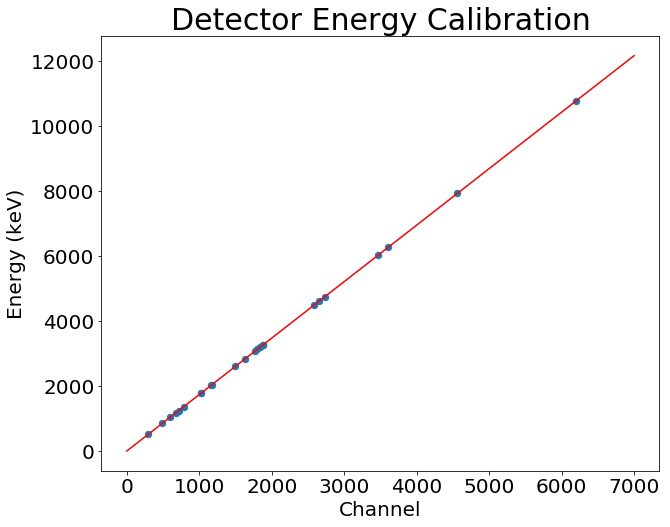
\includegraphics[width=0.8\linewidth]{figures/detEnergyCalibration.png}
\caption{Energy calibration curve for the HPGe detector taken at CASPAR. The calibration incorporated natural background, radioactive sources, and the products from the $^{27}$Al($p, \gamma$)$^{28}$Si reaction. }
\label{fig: energyCalibration}
\end{figure}





\section{Efficiency}
\label{sec: efficiency}

Efficiency is a term that can, in different contexts, have many different meanings. However, in experimental physics it is known to be the ratio for the response of an instrument to the actual physical quantity for which it is employed to measure. In these cases, it is the ratio between the photons recorded and those emitted in a given event. For this experiment, both the total efficiency, $\eta^{tot}$, and the full-energy peak (FEP) efficiency, $\eta^{fep}$, were required. The total efficiency is the probability that the $\gamma$ ray enters and deposits any amount of energy within the detector, while, on the other hand, the FEP efficiency is the probability that the full energy of an emitted $\gamma$ ray will be deposited within the detector. As both efficiency types are dependent on the physical geometry of the system, they are determined for each experimental setup in turn. 

\subsection{Total efficiency}
\label{subsec: totEff}

The total efficiency of a detector / source geometry is the probability that a given photon from the source will enter and deposit any amount of energy within the detector. For extremely simple geometries, the total efficiency can be calculated following the approach laid out in Debertin and Helmer \cite{DebertinHelmerBook},

\begin{equation}
\eta^{tot} = \dfrac{1}{4\pi} \int \left(1 - e^{-\mu x} \right) d\Omega
\end{equation}

\noindent where $\mu$ is the energy and absorber dependent attenuation coefficient, x is the position from the detector face, and the integration takes place over the solid angle of the detector from the front to the back. This formulation makes it abundantly clear that $\eta^{tot}$ is so highly dependent on the geometry of the setup. 

However, in practice, there is no analytic formulation of the total efficiency because one needs to account for any potential scattering of $\gamma$-rays off of any surrounding material, like the shielding or target chamber, for example. Additionally, when measuring the total efficiency for a given setup, the presence of multiple decays from physical sources provides additional complications. Therefore, most commonly the total efficiency is determined using single-line radioactive sources, like $^{137}$Cs, with well known activity. In this case, when accounting for the ever-present background, the total efficiency is the total number of counts in a spectrum divided by the total number of decays occurring during the measurement time, which can be easily calculated with the radioactive decay law

\begin{equation}
N(t) = N_{0} e^{- \lambda t} \hfill A(t) = A_{0} e^{- \lambda t},
\end{equation}

\noindent where $N(t)$ is the number of nuclei remaining after time $t$, $N_{0}$ is the initial number of radioactive nuclei, $\lambda$ is the radioactive decay constant for a given nucleus, $A(t)$ is the activity of the source at time $t$ compared to the activity at time $t=0$ of $A_{0}$. The decay constant, $\lambda$, can be calculated from either the nuclear lifetime, $\tau$, or the decay half-life, $t_{1/2}$, as

\begin{equation}
\lambda = \dfrac{1}{\tau} \hfill \lambda = \dfrac{\text{ln}(2)}{t_{1/2}}.
\end{equation}

\noindent This is how the total efficiency for the detector systems was determined at 662 keV, the $\gamma$ energy from the decay of $^{137}$Cs.



\begin{figure}
\centering
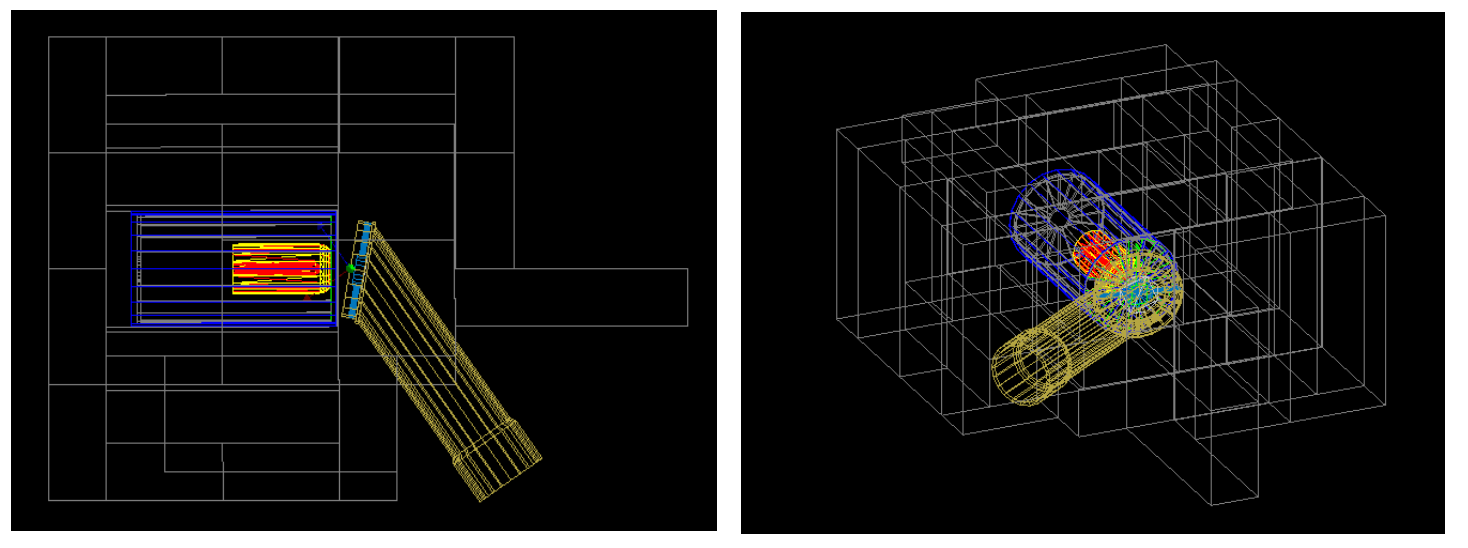
\includegraphics[width=\linewidth]{figures/shieldingSimulation.png}
\caption{Simulation of the experimental setup at CASPAR, including the target chamber (in gold), water cooling (in light blue), HPGe detector (in dark blue), and lead bricks for shielding (in gray). Both pictures are of the same experimental setup from different angles to convey the layout. Simulating this setup is necessary to determine the total efficiency of the experimental setup. In this determination, a single-line $\gamma$ source is placed at the target location and its decays simulated for a variety of energies, allowing a determination of the total efficiency at each.}
\label{fig: simulatedSetup}
\end{figure}


\begin{figure}
\centering
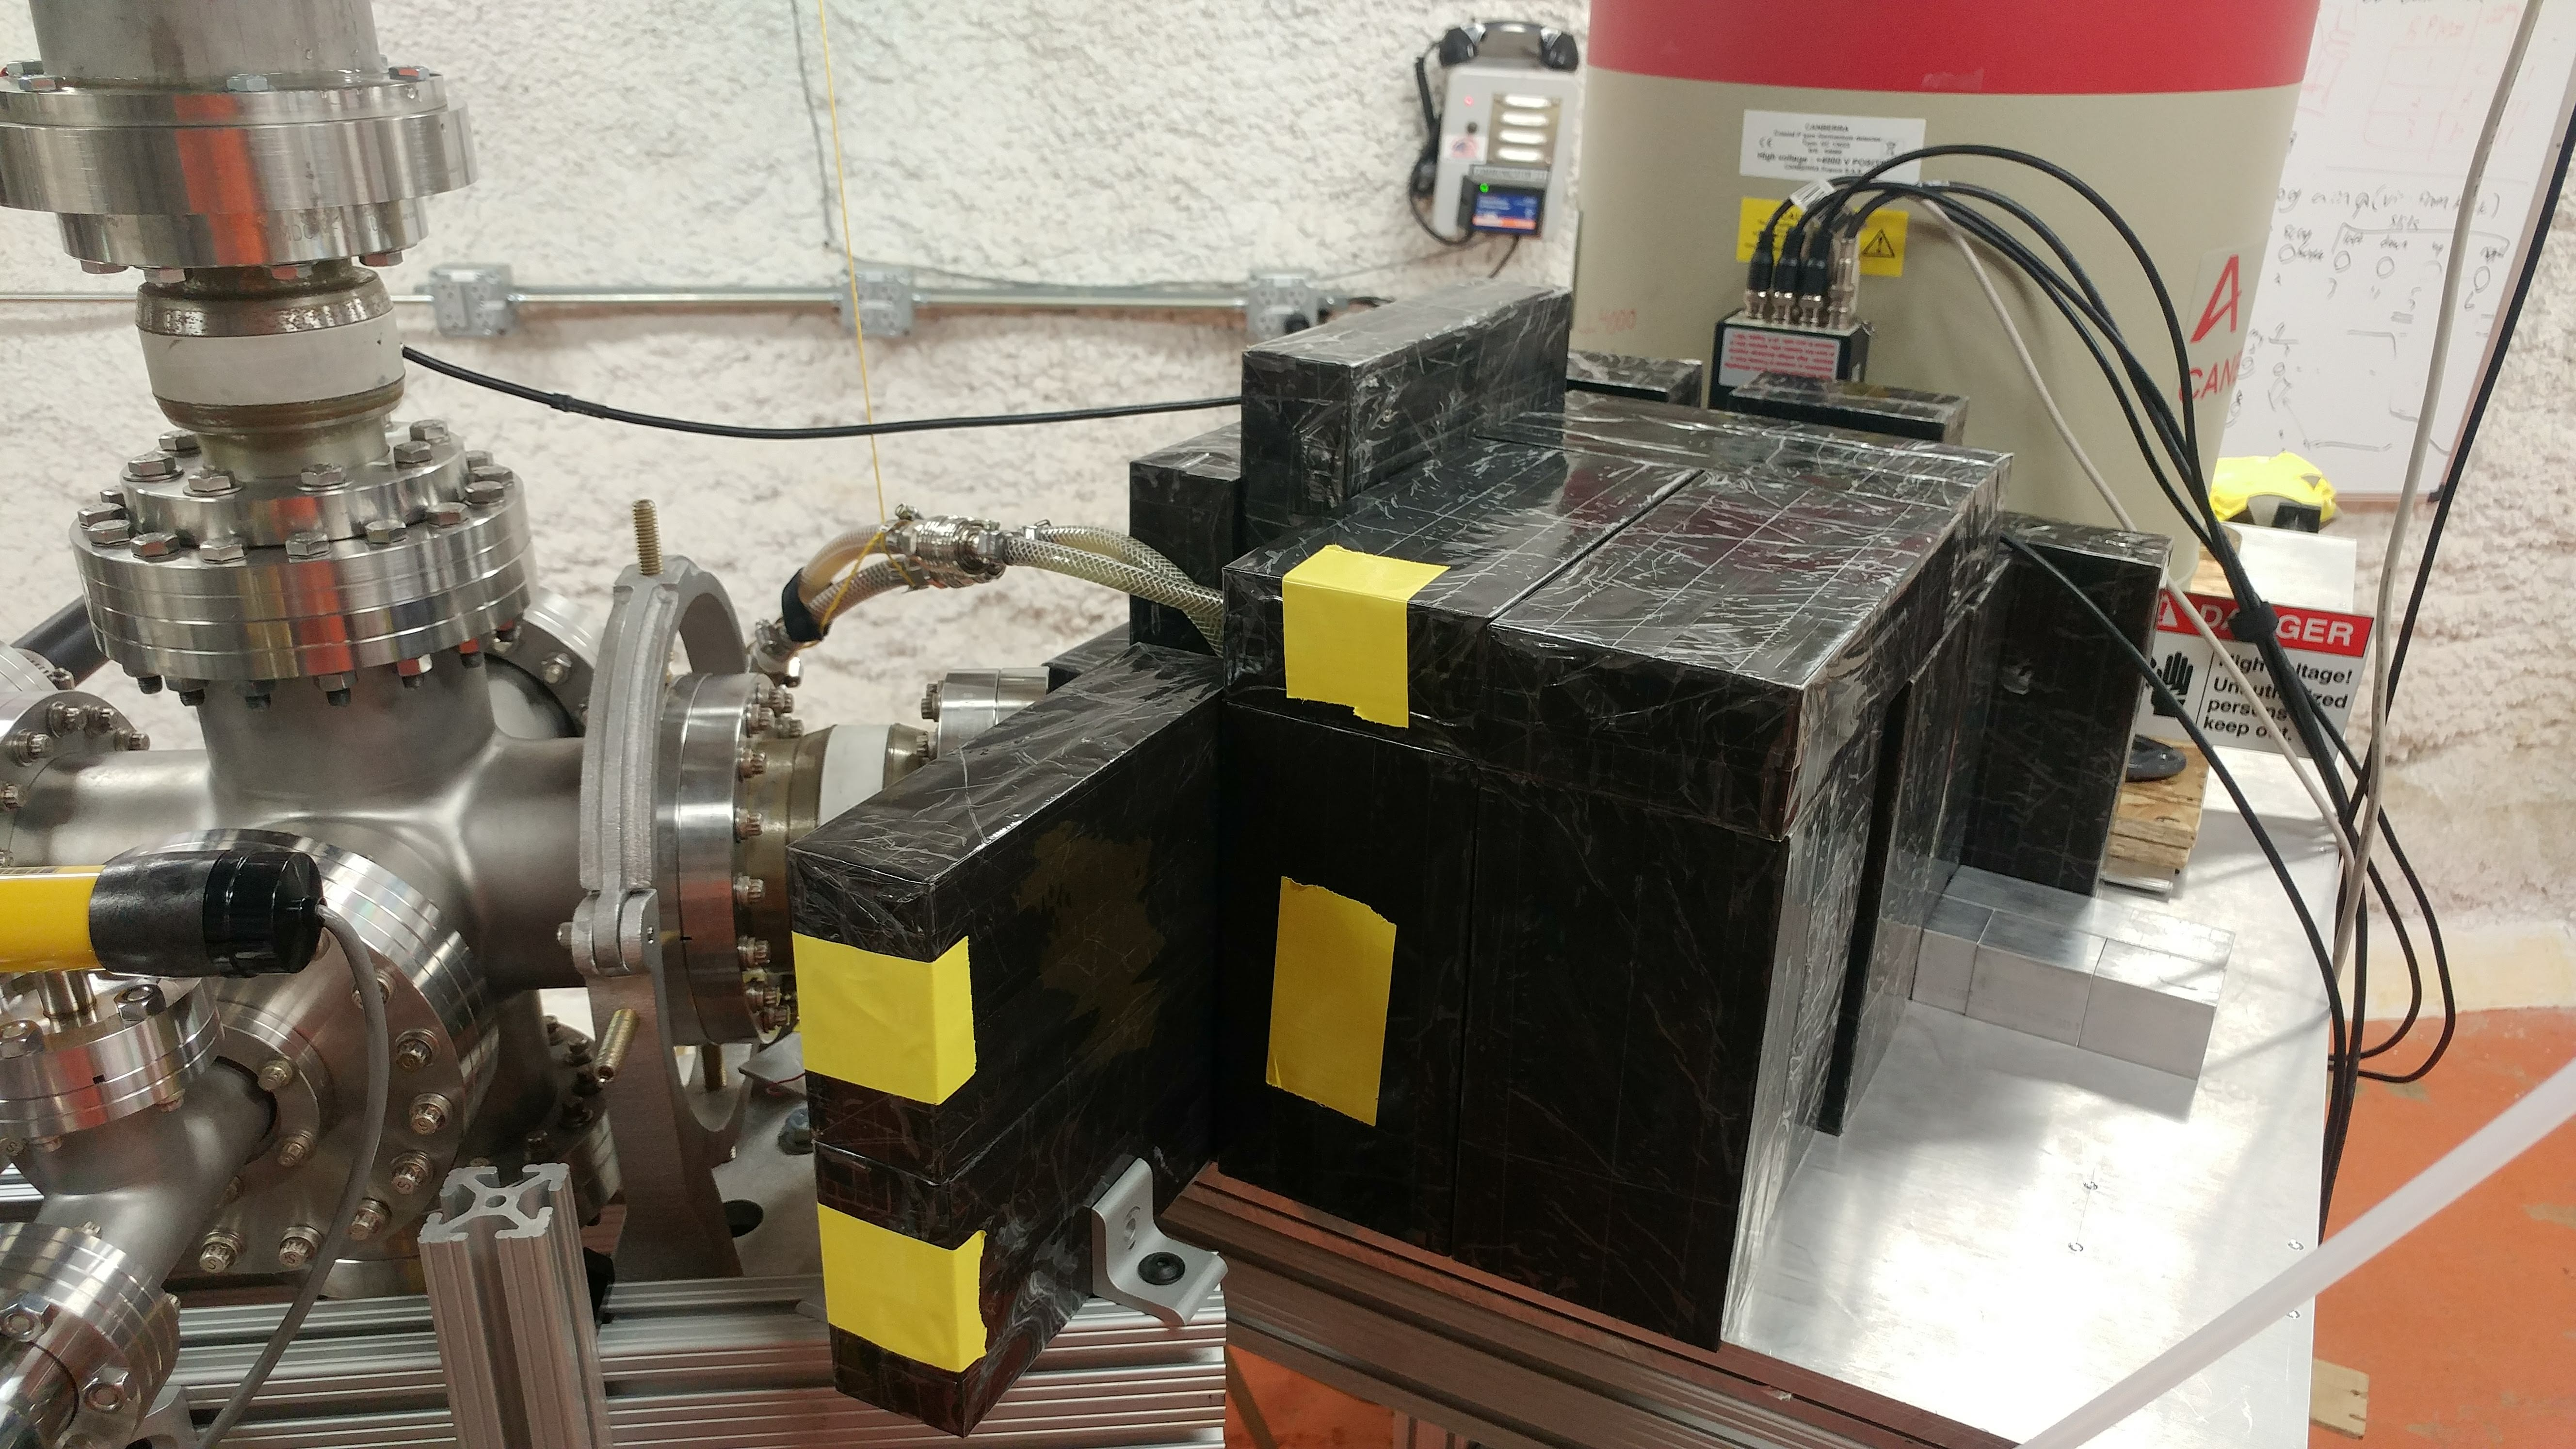
\includegraphics[width=0.8\linewidth]{figures/shieldingPicture.jpg}
\caption{A picture of the experimental setup at CASPAR, showing the lead shielding around the detector and target chamber. This figure is provided for comparison to the simulated setup to prove its accuracy. }
\label{fig: actualSetup}
\end{figure} 

To extend $\eta^{tot}$ to the whole range of energies relevant to the experiments, the experimental setup (including the target chamber, water cooling, and shielding) was built and simulated in Geant4 \cite{Agostinelli2003}, an example of the simulation for the CASPAR setup is shown in Fig.\ \ref{fig: simulatedSetup} where the actual setup is given in Fig.\ \ref{fig: actualSetup} for comparison. Then, a single-line emission source was recreated at the target location and simulated 10,000,000 decays, recording the deposited energy inside the detector. The energy of the source was changed and simulated at energies of 662, 1300, 2000, 3000, 4000, 6000, 7000, 8000, and 10000 keV to cover the entire range of $\gamma$ ray energies present in the $^{14}$N$\left( p,\gamma \right) ^{15}$O reaction. For each of the different decay energies, the spectrum of recorded events in the detector was analyzed in the exact same way as the actual $^{137}$Cs data to produce the total efficiency at each energy. This simulated data was used in conjunction with the measured $^{137}$Cs total efficiency data point to determine an accurate curve of the total efficiency across all experimentally relevant energies, shown in Fig.\ \ref{fig: totalEfficiency}.

\begin{figure}
\thisfloatpagestyle{plain}
\centering
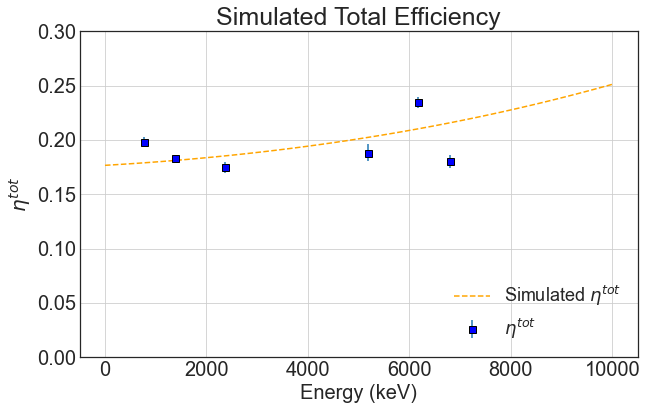
\includegraphics[width=\linewidth]{figures/totalEfficiency.png}
\caption{The total efficiency of the HPGe in the CASPAR setup across all relevant energies. The points from the Geant4 simulation are taken raw without scaling, showing the efficacy of this technique and accuracy of the simulation. Further details about the calculation of these curves can be found in Sec. \ref{subsec: totEff}. \textbf{I'M PRETTY SURE I'VE MADE AN UPDATED VERSION OF THIS FIGURE BUT I WASN'T ABLE TO EASILY FIND IT. I'LL KEEP LOOKING THOUGH.}}
\label{fig: totalEfficiency}
\end{figure}



\subsection{Peak efficiency}

The full energy peak (FEP) efficiency, on the other hand, is the probability that the full energy of a given photon will be recorded within the detector. Mathematically, this is

\begin{equation}
\eta^{FEP} = \dfrac{n(E)}{R(E)}
\end{equation}

\noindent where $n(E)$ is the count rate in the measured peak at an energy, $E$, where $R(E)$ is the rate at which photons of energy $E$ are emitted from the source \cite{DebertinHelmerBook}. From this point, if not specified, efficiency as a term is used to denote the FEP efficiency whereas the total efficiency will always be named explicitly. 

Determining the efficiency for a given setup is necessary for each geometry since, like the total efficiency, it is related to the specific source-detector geometry; it is not an intrinsic property of a given detector. In this campaign of experiments, the efficiency was determined each time with a combination of radioactive sources, like $^{137}$Cs, $^{60}$Co, and $^{152}$Eu, and well-known nuclear resonances, like $^{14}$N$\left( p,\gamma \right) ^{15}$O at $E_{p}$ = 278 keV and the $^{27}$Al($p, \gamma$)$^{28}$Si resonance at $E_{p}$ = 992 keV. These reactions were chosen because, much like the energy calibration, these extend the detector's measured efficiency to a much higher energy range (up to 10.7 MeV) compared to radioactive sources. 

From radioactive sources, the detector's efficiency at a given $\gamma$ ray energy, $\eta(E_{\gamma})$, can be determined with

\begin{equation}
\eta (E_{\gamma}) = \dfrac{N_{\gamma}}{A(t) B_{\gamma} t_{live} C_{i}},
\end{equation}

\noindent where $N_{\gamma}$ is the measured number of counts in the full energy peak, $A(t)$ is the source's activity at the time of the measurement, $B_{gamma}$ is the branching ratio for the specific decay, $t_{live}$ is the live time of the measurement, and $C_{i}$ are the correction factors, if necessary. For nuclear resonances, on the other hand, $\eta (E_{gamma})$ is 

\begin{equation}
\eta (E_{\gamma}) = \dfrac{N_{\gamma}}{q B_{\gamma} R C_{i}},
\end{equation}

\noindent where $q$ is the collected charge and

\begin{equation}
R = \dfrac{\lambda_{r}^{2}}{\pi} \dfrac{\omega \gamma}{\epsilon_{sp}} \dfrac{M + m}{M} \tan^{-1} \left( \dfrac{\Delta E}{\Gamma}  \right)
\label{eqn: resonanceFactor}
\end{equation}

\noindent with $\lambda_{r}$ is the proton's de Broglie wavelength at the resonance energy, $\omega \gamma$ is the resonance strength (as defined in Chapter \ref{chap: introduction}), $\epsilon_{sp}$ is the stopping power of the target at the resonance energy, $M$ is the target atomic mass, $m$ is the projectile atomic mass, $\Delta E$ is the thickness of the target, and $\Gamma$ is the resonance width. 

For this determination, the branching ratios for the 278 keV resonance in $^{14}$N$\left( p,\gamma \right) ^{15}$O were taken from Daigle \textit{et al.} \cite{Daigle2016} where for the 992 keV resonance in $^{27}$Al($p, \gamma$)$^{28}$Si they were obtained from Antilla \textit{et al.} \cite{Antilla1977} and those from the 406 keV resonance in $^{27}$Al($p, \gamma$)$^{28}$Si are taken from Powell \textit{et al.} \cite{Powell1998}. The efficiencies were then fit with 

\begin{equation}
\eta = \exp \left(  \sum_{i=0}^{3} a_{i} ( \ln (E_{\gamma}))^{2}    \right),
\end{equation}

\noindent where the $a_{i}$ are fit coefficients and $E_{\gamma}$ is the $\gamma$-ray energy and the independent variable in the fit. An example of this determination for the CASPAR setup in both the close and far geometries can be seen in Fig. \ref{fig: efficiency}. In both calculations, only statistical errors were included in the fit and the highest energy point was excluded due to summing effects, which will be discussed in more detail in the next section. This can be clearly seen as the highest energy point at close distance (1.1 cm from target) is off by an inordinately large factor. For a reference, measurements were also taken at 25.24 cm away from the target chamber, making the summing effects negligible. In this case, the summing effects provide very little impact (if any) on the highest energy point, which was still excluded from this fit. However, for the far distance it follows the trend of the other data nearly perfectly.


\begin{figure}
\centering
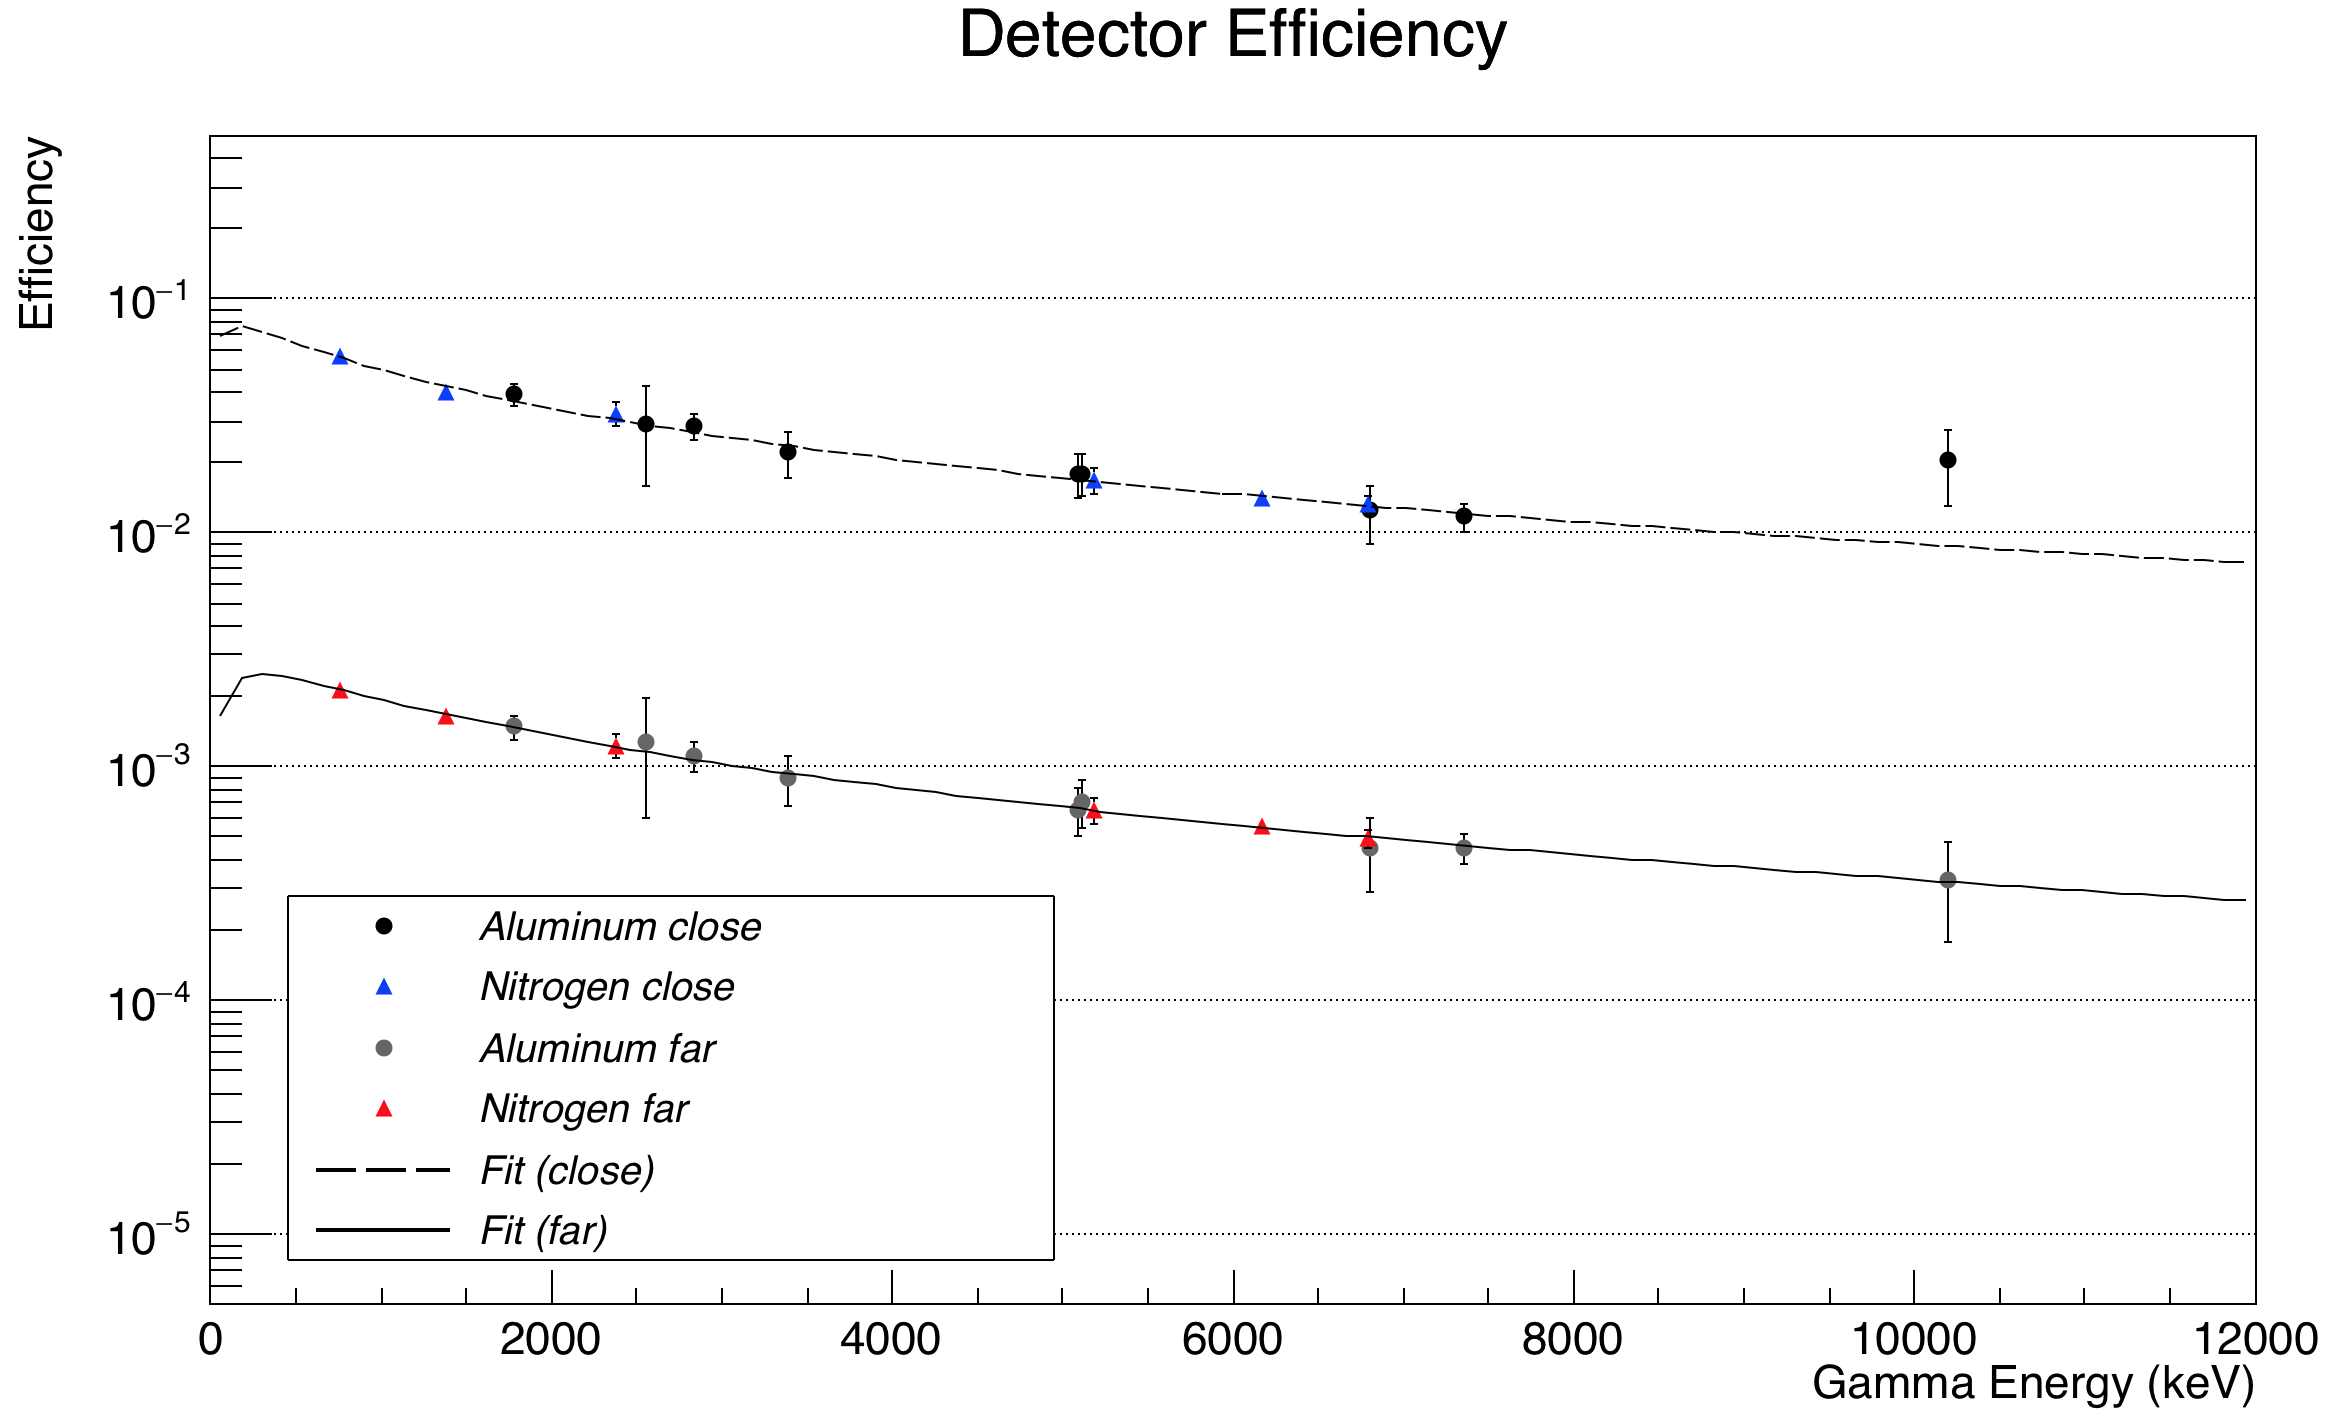
\includegraphics[width=\linewidth]{figures/efficiencyComplete.png}
\caption{Detector efficiency as a function of $\gamma$-ray energy for the measurement at CASPAR in both close and far geometries. The highest energy point in the close geometry was excluded from the fit because it suffers from summing-in effects artificially inflating the count rate of this measured peak (see text for details). At the far distance between the detector and the target, summing effects are negligible.   }
\label{fig: efficiency}
\end{figure}



\section{Summing corrections}
\label{sec: summing}

Summing corrections need to be applied to data due to data-recording phenomena manifesting in measured spectra. There are two different ways in which the recorded data can be affected, the so-called summing-in and summing-out effects, and these are more pronounced when measurements happen with the detector and source in close proximity or with simple reaction product decay structures, as in the case in the $^{14}$N$\left( p,\gamma \right) ^{15}$O reaction.


\begin{figure}
\centering
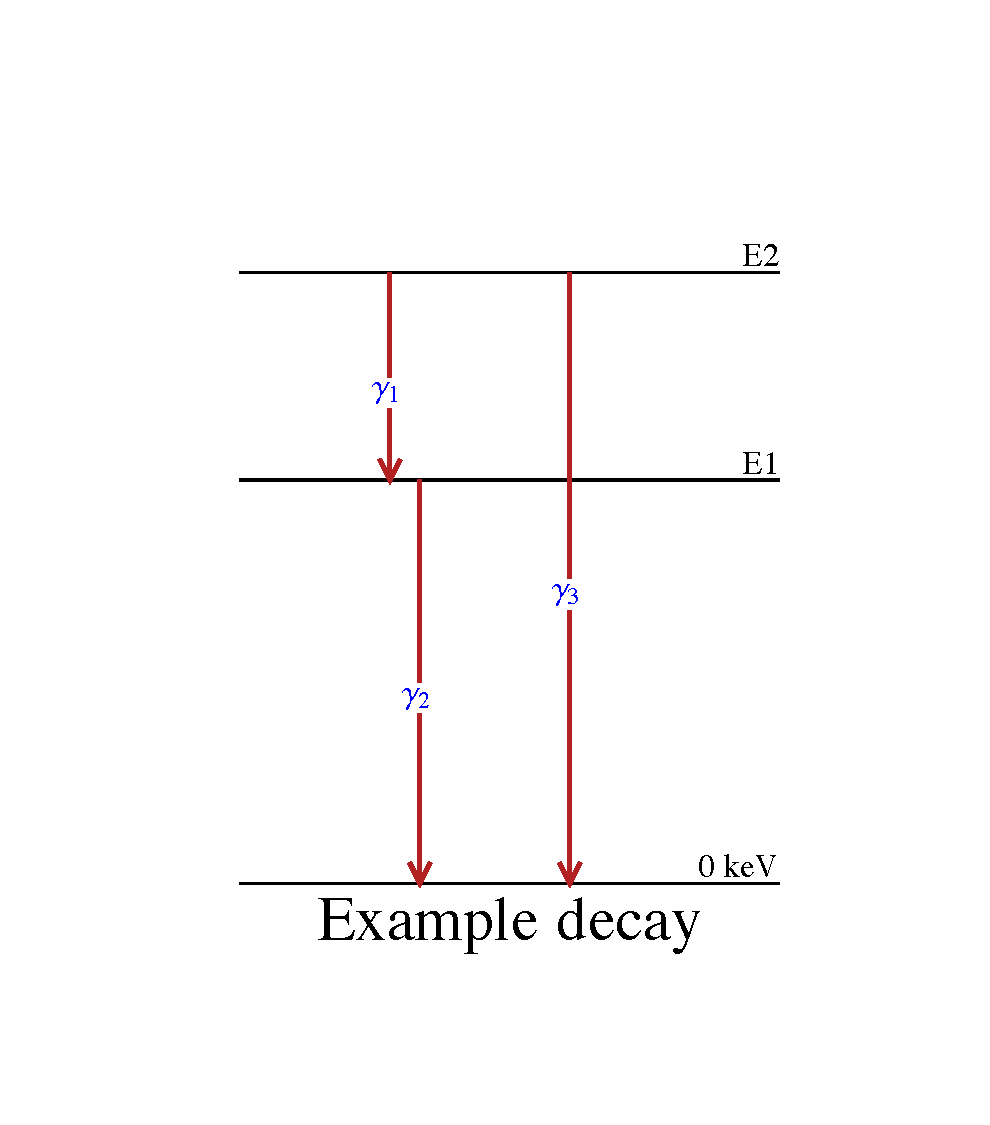
\includegraphics[width=0.7\linewidth]{figures/simpleScheme.pdf}
\caption{Example cascade nuclear decay for demonstrating summing effects (see text for details). }
\label{fig: simpleDecay}
\end{figure}

For a simple nuclear decay, like that in Fig. \ref{fig: simpleDecay}, summing manifests in a measured spectrum in two different ways. If any portion of the energy from $\gamma_{1}$ is deposited in the detector simultaneous with $\gamma_{2}$, the the resultant recorded event will have an energy higher than either individual $\gamma$-ray and, therefore, will appear at a different energy in the spectrum. Consequently, $\gamma_{2}$'s count rate will be artificially lowered. By the same logic, the count rate for $\gamma_{1}$ will also be artificially dropped. This loss of counts in the peaks recorded at energies $E_{1}$ and $E_{2}$ is known as the summing-out effect. As an extension of this thought experiment, if the full energy of both $\gamma_{1}$ and $\gamma_{2}$ is deposited in the detector at the same time the resulting measured energy will match $E_{3}$, artificially inflating the count rate of that peak. This increase is called the summing-in effect.

To correct for these effects, the probability of measuring a different energy than expected must be taken into account. For a situation where there is no summing, the rate of $\gamma$ rays is simply the yield

\begin{equation}
Y_{i} = R B_{i} \eta_{i},
\end{equation}

\noindent where $R$ is the normalization from Equation \ref{eqn: resonanceFactor}, $B$ is the branching ratio, and $\eta$ is the FEP efficiency. However, when summing-out occurs, the yield is artificially dropped by the factor $R B \eta_{1} \eta^{tot}_{2}$, which is the probability of counting the full energy of $\gamma_{1}$ along with any part of $\gamma_{2}$. Mathematically, this observed yield for both $\gamma_{1}$ and $\gamma_{2}$ is

\begin{align}
Y_{1} &= R B_{1} \eta_{1} - R B_{1} \eta_{1} \eta^{tot}_{2} \\
        &= R B_{1} \eta_{1} \left( 1 - \eta^{tot}_{2} \right) \\
Y_{2} &= R B_{2} \eta_{2} \left( 1 - \eta^{tot}_{1} \right).
\end{align}

\noindent Then, in order to correct for this, the ratio of the true emitted $\gamma$'s to the observed rate for $\gamma_{1}$ is

\begin{equation}
\dfrac{Y_{1}}{Y^{obs}_{1}} = \dfrac{1}{1 - \eta^{tot}_{2}} = C_{1},
\end{equation}

\noindent where the $C_{i}$ is the correction factor. The same relation holds for $\gamma_{2}$. This makes clear why the total efficiency is so important: without it, summing-out is not an effect which can be corrected. For $\gamma_{3}$, however, the situation requires the total energy deposition of $\gamma_{1}$ and $\gamma_{2}$ at the same time, so correcting for summing-in requires the FEP efficiency. This is

\begin{equation}
Y_{3} = R B_{3} \eta_{3} + R B_{1} \eta_{1} \eta_{2}
\end{equation} 

\noindent where the second term includes $B_{1}$ because the decay chain has to start with $\gamma_{1}$. By the same token, the correction factor for summing-in is

\begin{equation}
C_{3} = \dfrac{Y_{3}}{Y_{3}^{obs}} = \dfrac{1}{1 + \left( \dfrac{B_{1} \eta_{1} \eta_{2}} {B_{3} \eta_{3}}  \right)}.
\end{equation}


With a more complicated nuclear level scheme, the summing corrections become more difficult to apply accurately. A more detailed treatment of the necessary methods can be found in \cite{DebertinHelmerBook}. This is primarily due to more complicated feeding and the presence of multiple decays from a given level. In general, the correction is for the $i$th level is

\begin{align}
C_{i} &= 1 + C_{i}^{in} - C_{i}^{out} \\
C_{i}^{in} &= \sum_{m,n} \dfrac{B_{m} p_{n} \eta_{m} \eta_{n}}{B_{i} \eta_{i}} \\
C_{i}^{out} &= \sum_{j,k} p_{k} \eta_{k}^{tot} + \dfrac{B_{j} p_{i} \eta_{j}^{tot}}{B_{i}}
\end{align}




\begin{figure}
\thisfloatpagestyle{plain}
\hspace{-2cm}
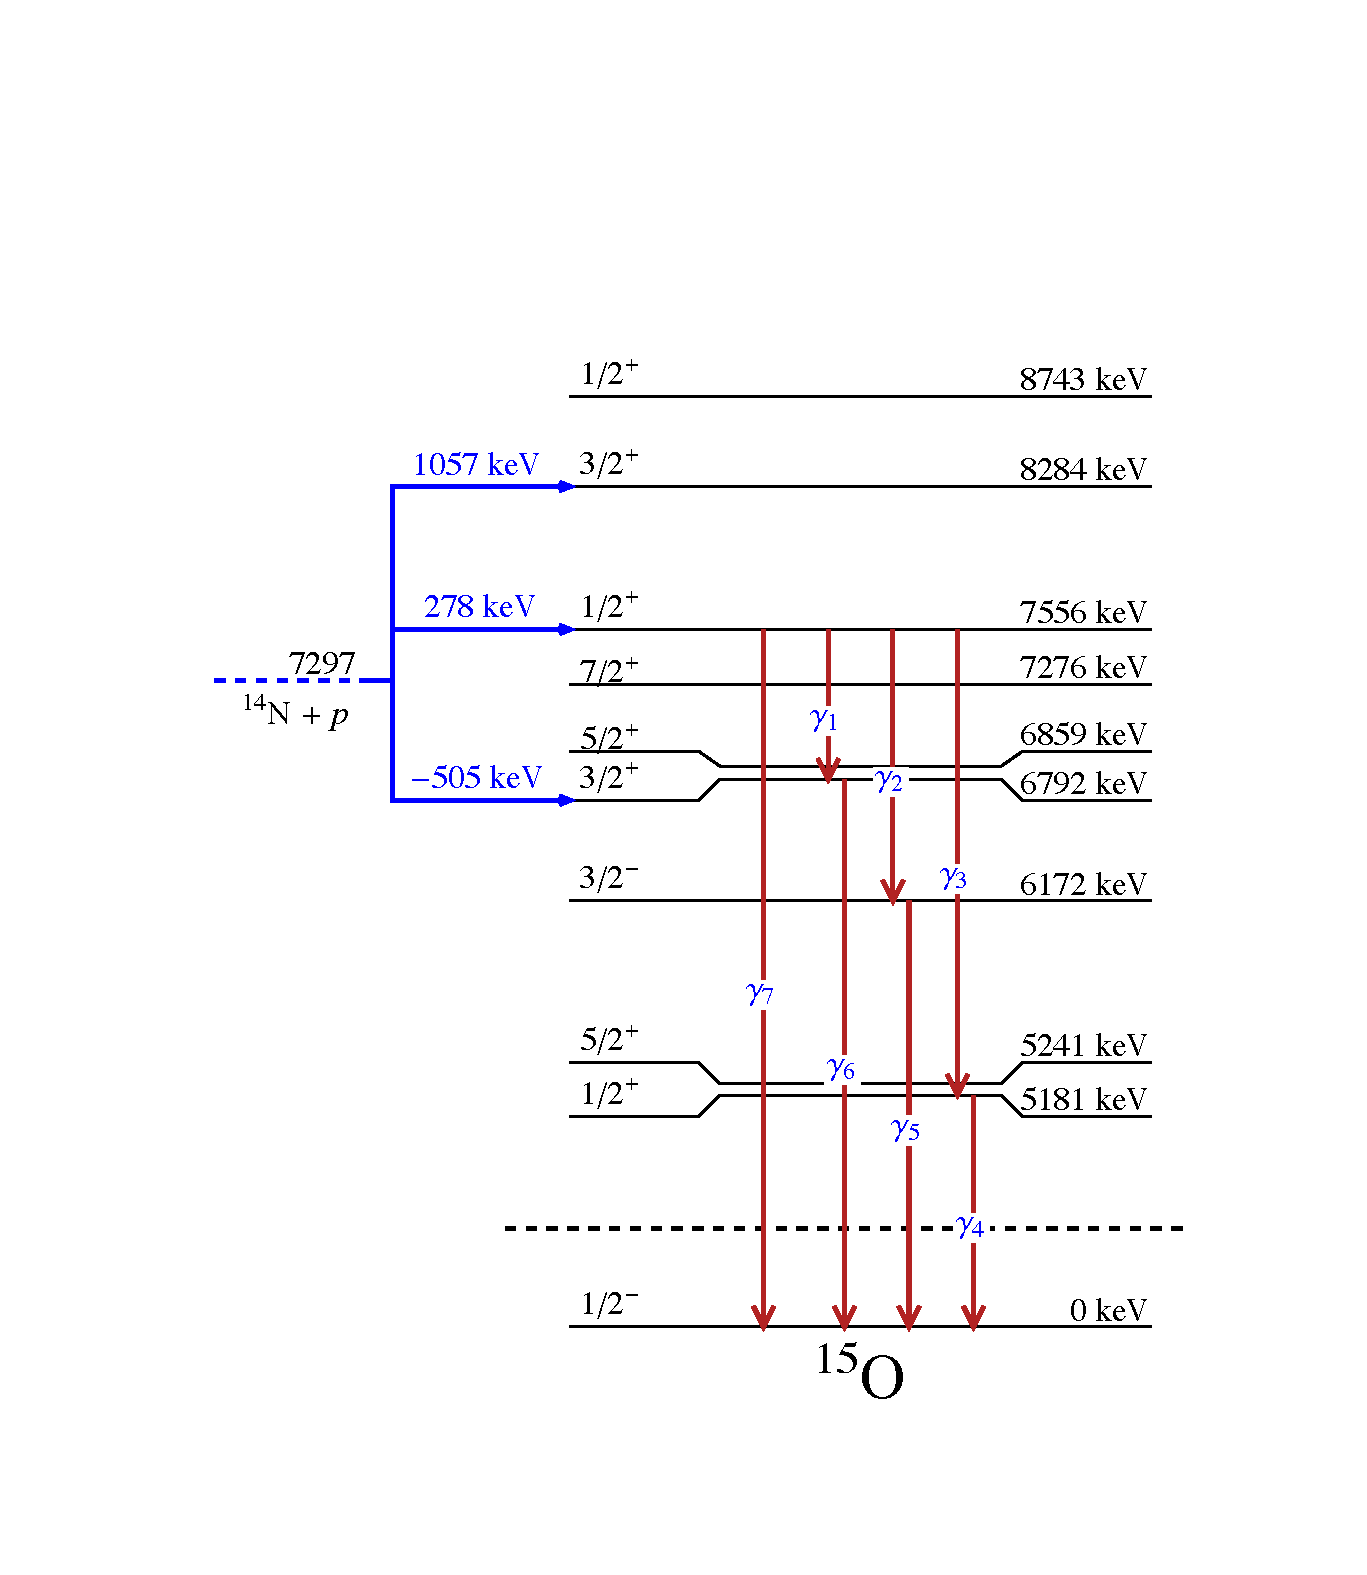
\includegraphics[width=1.0\linewidth]{figures/summingOxygenDecays.pdf}
\caption[All decays from the 278 keV proton resonance in the $^{14}$N$\left( p,\gamma \right) ^{15}$O reaction. Other than the resonance level, all decays are sequential, with the levels having only one decay directly to ground state. Of note, this then means that the total energy for each decay sequence matches the direct transition, $\gamma_{7}$, so it must be corrected for summing-in effects from all the other branches.]
{{\small All decays from the 278 keV proton resonance in the $^{14}$N$\left( p,\gamma \right) ^{15}$O reaction. Other than the resonance level, all decays are sequential, with the levels having only one decay directly to ground state. Of note, this then means that the total energy for each decay sequence matches the direct transition, $\gamma_{7}$, so it must be corrected for summing-in effects from all the other branches. }}
\label{fig: summingOxygen}
\end{figure}

\noindent where the $p_{i}$ are the probability of feeding. Fortunately, for the $^{15}$O nucleus, all intermediate decays have a branching ratio of 100\%, as can be seen in Fig.\ \ref{fig: summingOxygen}. The summing out corrections in each case can then be

\begin{equation}
C_{i}^{out} = 1 - \eta^{tot}_{j},
\end{equation}

\noindent where the $i$ and $j$ denote the $\gamma$ rays feeding into and decaying from the state, respectively (like $\gamma_{1}$ and $\gamma_{6}$ for example). For this measurement, the summing-out effect for every transition falls in the range of 28 - 32 \% for all of the relevant $\gamma$'s. %Fig.\ \ref{fig: sumOutRange} shows this, depicting the summing out correction across the range of relevant gamma energies in this experiment. 


%\begin{figure}
%		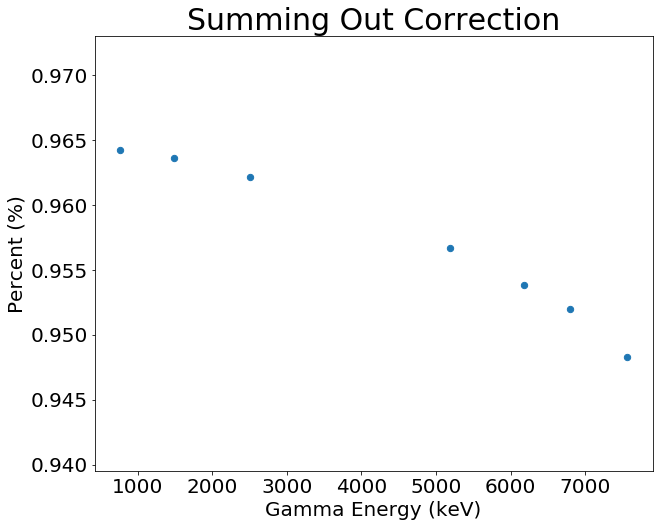
\includegraphics[width=1.0\linewidth]{figures/sumOutRange.png}
%	\caption[The summing out correction as a function of incident $\gamma$-ray energy. This figure shows the percentage of gammas recorded to the true incident number.]
%	{{\small The summing out correction as a function of incident $\gamma$-ray energy. This figure shows the percentage of gammas recorded to the true incident number.}}
%	\label{fig: sumOutRange}
%\end{figure}


Conversely, only the R/DC$\rightarrow$GS transition needs to be corrected for summing-in effects as the total energy of the other decay branches matches the energy of $\gamma_{7}$, and, as such, should be a larger effect since the true branch to the ground state is $\sim 1.5$\% \cite{Daigle2016}. The observed yield of $\gamma_{7}$ in this case will be

\begin{equation}
Y_{7} = R B_{7} \eta_{7} + R B_{1} \eta_{1} \eta_{6} +  R B_{2} \eta_{2} \eta_{5} + R B_{3} \eta_{3} \eta_{4} .
\end{equation}

\noindent From this, then, the correction factor for the ground state transition will necessarily be

\begin{equation}
C_{7}^{in} = 1 + \dfrac{B_{1} \eta_{1} \eta_{6} + B_{2} \eta_{2} \eta_{5} + B_{3} \eta_{3} \eta_{4} }{B_{7} \eta_{7}}.
\end{equation}

\noindent In this measurement, this correction is quite large, as expected. It was determined to be a 61\% correction to the ground state transition using this method. \textbf{THIS NUMBER NEEDS TO BE UPDATED WHEN I HAVE FIXED THIS CALCULATION. I EXPECT SOMETHING IN THE RANGE OF 70-80 PERCENT AND IT CURRENTLY CALCULATES TO 15. ONCE THESE AGREE, I CAN PROCEED.}

There is a second method for calculating the summing-in correction which was also employed. This relies on the measured efficiency being taken at different distances to the source of the $\gamma$ rays. In close geometry, the solid angle of the detector is much larger when viewed from the source and summing is present (which can be seen from the highest energy data point in the detector efficiency plot, Fig.\ \ref{fig: efficiency}). However, at a larger distance, in this case 25.4 cm, the solid angle of the detector is significantly smaller but summing-in effects are not present in the detector. Therefore, the ratio of efficiencies between the close and far distance measurements when accounting for the difference in detector solid angle is the necessary summing-in correction. 


\begin{figure}
\centering
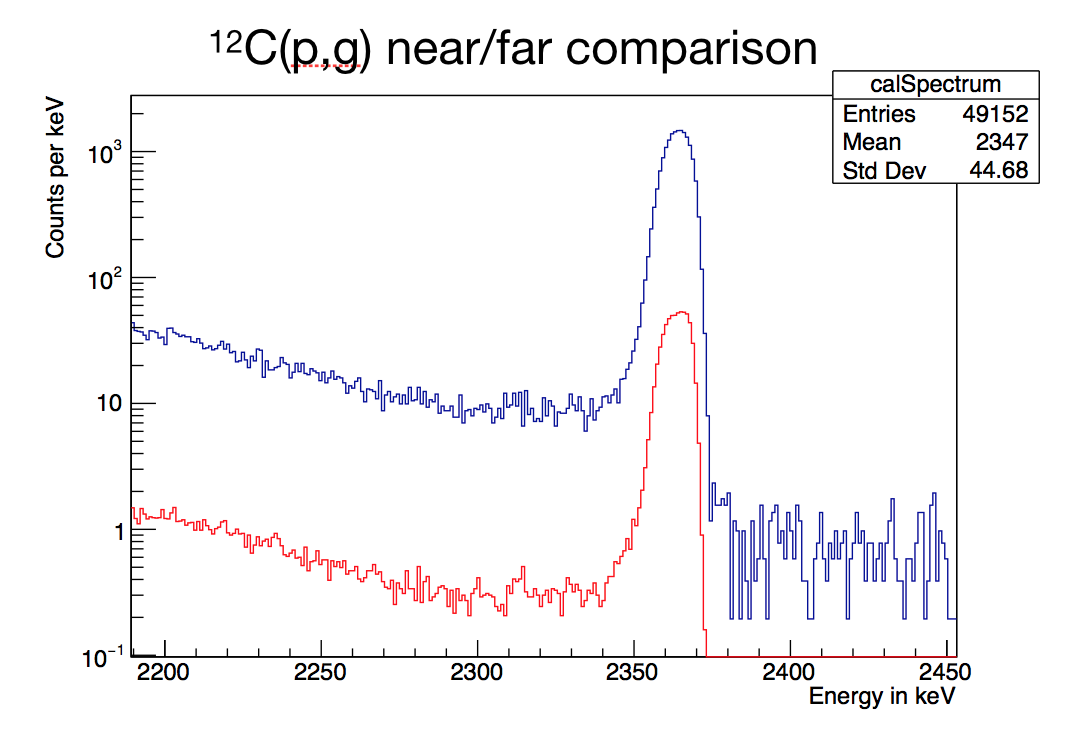
\includegraphics[width=\linewidth]{figures/carbonComparison.png}
\caption{Spectra from the $^{12}$C$\left( p,\gamma \right) ^{13}$N reaction obtained at CASPAR. The ratio of counts in the near (blue) and far (red) spectra gives us a ratio with which to correct between the near/far efficiencies. }
\label{fig: 12cpg}
\end{figure}

More accurately than calculating the solid angle geometrically, the near/far correction factor can be determined using another set of measurements with the $^{12}$C$\left( p,\gamma \right) ^{13}$N reaction. For this method, the reaction decays via a single $\gamma$ at 2.37 MeV and requires no additional correction for summing. This means that the difference between the data taken in near/far distances is due to the geometric effects and allows us to relate the efficiencies between the two measurement distances without the need for correcting for summing-out or summing-in. Spectra from the $^{12}$C$\left( p,\gamma \right) ^{13}$N reaction taken at CASPAR are shown in Fig.\ \ref{fig: 12cpg}. The ratio of counts in these two peaks gives a near/far ratio of $R_{c} = 27.8$. Using this ratio, we scale up the fitted far-efficiencies and the difference between this and the ground state peak provides the needed summing-in correction. For our data, the summing-in correction was found to be 74.6\% for the ground state transition. 



The fact that these two methods give nearly the same value for the summing-in serves as good cross-validation of these corrections. When incorporating this result into the final cross section determination, the mean of these two correction values was taken, at 75\%. 






\section{Target characterization}
\label{sec: targetCharacterization}

In order to ultimately determine the nuclear cross section and the astrophysical $S$-factor for a given reaction, the number of active atoms in the target must be known. As a reminder, the nuclear cross is a probability of interaction. The number of possible reaction sites must be known. The targets used in these measurements were sputtered TiN and ZrN targets, backed by Ta and W, respectively. By performing an energy scan over a known, thin resonance with the targets it is possible to determine the number of active atoms in the target. 

Fig. \ref{fig: yieldRes} presents a typical example of a resonance scan, which is just the measured excitation function over a resonance. This one was taken at CASPAR with the 278 keV resonance in $^{14}$N$\left( p,\gamma \right) ^{15}$O with ZrN target (\# 5) by monitoring the R $\rightarrow$ 6.79 MeV transition. Even for a monoenergetic beam, there is still a small gaussian distribution of energies encompassed in the beam (see Chapter \ref{chap: experiment} for more details). When the high energy tail of this distribution reaches the low energy side of the resonance, the measured yield from that resonance will appear. Further increasing the beam energy implies that more of the energy distribution of the beam reaches the resonance energy and the yield continues to increase. This low-energy side of the scan is referred to as the front edge and contains the intrinsic information about the resonance as well as the beam distribution. The true resonance energy, $E_{r}$ is found halfway up the front edge, 50\% of the maximum yield, because at this point a symmetric beam distribution would be half above and half below the resonance in energy. Similarly, the slope of the front edge details the energy spread in the beam, with a broader distribution corresponding to a lower slope and a tighter distribution providing a sharp front edge. 

For the incident beam particles that are above the resonance energy, they will lose energy traveling through the target and drop to energies within the resonance width and proceed through resonant capture. The maximum yield for such a scan will occur when the entire beam distribution is at an energy such that either a maximum of the ions are within the resonance width or the energy loss in the target brings a maximum number of the ions into that same range.  This maximum is known as the plateau and is the flat portion at the top of the curve in Fig. \ref{fig: yieldRes}. As a target's thickness increases the thicker this plateau becomes, since the ions will have a greater energy loss within the active target material, allowing them to decrease to resonance energy from higher and higher starting energies. For an infinitely thick target, the resonance plateau would never decrease again on the high side, because the beam would always lose enough energy to fall back into the resonance while still in the active target material. 

When targets are not infinitely thick, however, the beam energy can be increased to a point where the energy loss of the ions will eventually be such that the energy of the ions is still above the resonance width when leaving the active target material, meaning the reaction no longer proceeds through the resonant capture mechanism. When this happens, the yield starts to decrease from the level of the plateau. By a similar argument to the beam distribution leading to increased yield on the front edge, the yield on the back edge (where the plateau decreases again) drops because of the same distribution effects. The slope of this decrease is affected by the target material (leading to different energy losses) and the homogeneity (or lack thereof) of the active material. The full-width half-maximum (FWHM) of this excitation curve represents the target thickness in terms of energy loss, $\Delta E$. 



\begin{figure}
\thisfloatpagestyle{plain}
		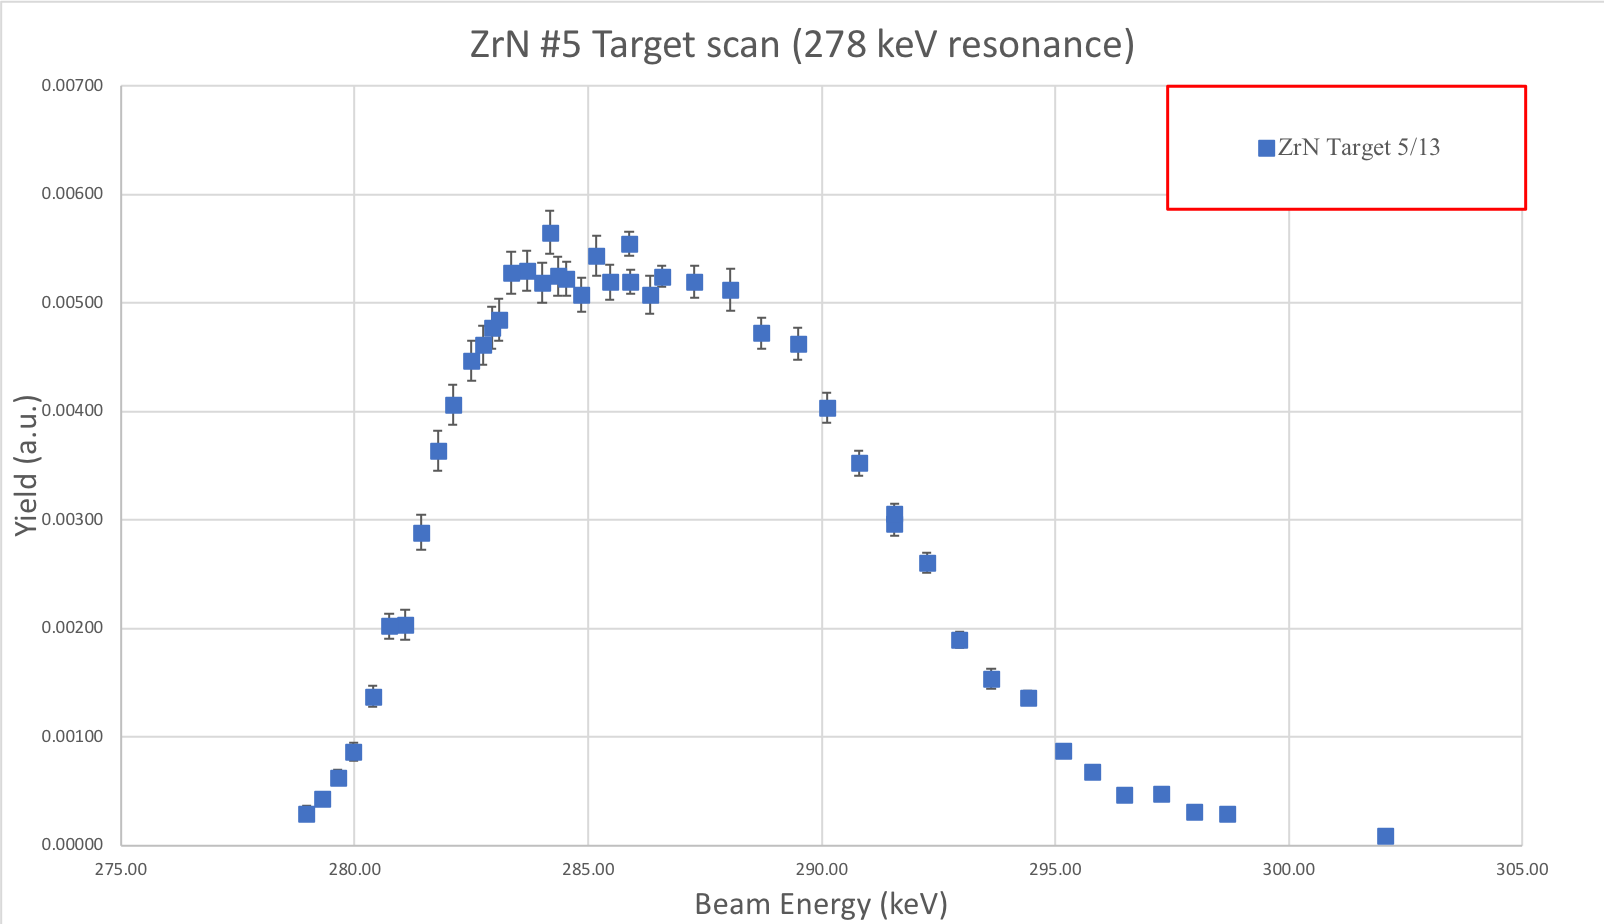
\includegraphics[width=1.0\linewidth]{figures/resScan.png}
	\caption{Resonance scan (measured Excitation curve over a resonance) taken at CASPAR with the 278 keV resonance in $^{14}$N$\left( p,\gamma \right) ^{15}$O with ZrN target (\# 5). This shows typical behavior of an energy scan over a thin resonance and from a measurement like this, the number of nitrogen atoms in the target can be determined (see text for details).}
	\label{fig: yieldRes}
\end{figure}


%There are two main methods by which the number of active atoms in a target can be determined, both of which rely on experimental scans over a thin resonance.  The targets used in these measurements were sputtered TiN and ZrN targets backed with Ta and W. 

For such a thin resonance occurring at $E_{r}$, the stopping power of the target, $\epsilon(E)$, the de Broglie wavelength, $\lambda$, and the partial widths $\Gamma_{i}$ do not change appreciably over the resonance energy. This allows the maximum yield, at $E_{0}$, to be calculated using \cite{IliadisBook}

\begin{align}
Y(E_{0}) &= \int_{E_{0}-\Delta E}^{E_{0}} \dfrac{1}{\epsilon(E)} \dfrac{\lambda^{2}}{4 \pi} \omega \dfrac{\Gamma_{a}\Gamma_{b}}{(E_{0}-E)^{2} = \Gamma^{2}/4} dE \\
           &= \dfrac{\lambda_{r}^{2}}{2 \pi} \dfrac{\omega \gamma}{\epsilon_{r}} \left[ \tan^{-1} \left(\dfrac{E_{0} - E_{r}}{\Gamma/2}  \right) - \tan^{-1} \left(  \dfrac{E_{0} - E_{r} - \Delta E}{\Gamma/2} \right)  \right].
\end{align}

Then, with some further algebraic reduction \cite{IliadisBook}, one can show

\begin{align}
E_{0} &= E_{r} + \dfrac{\Delta E}{2} \\
 Y_{max} &= \dfrac{\lambda_{r}^{2}}{\pi} \dfrac{\omega \gamma}{\epsilon_{r}} \arctan \left(\dfrac{\Delta E}{\Gamma} \right) \\
 FWHM &= \sqrt{\Gamma^{2} + \Delta E^{2}} \\
 n &= \dfrac{\Delta E}{\epsilon_{r}}, \label{eqn: targetNuclei1}
\end{align}

\noindent where $n$ is the number density of target atoms, atoms per unit area. When the target thickness, $\Delta E$ is much bigger than the resonance width, $\Gamma$, the FHWM of the resonance scan is simply the target thickness. Thus, by selecting thin resonances and determining the energy loss from their scans, like that in Fig.\ \ref{fig: yieldRes}, the number density of of active nuclei in the target can be determined with Equation \ref{eqn: targetNuclei1}. This method is useful because it does not rely on any external efficiency calibrations or corrections (since such a correction would apply to the entire curve equally, not changing the FWHM and, therefore, the thickness). Thus, this method is effective and appropriate for a uniform target material with known stoichiometry. 

The stopping powers used for these determinations were calculated using the James F. Ziegler's industry standard SRIM program, \cite{Ziegler2010}. The output from this program provides the discrete values for the stopping power of a user specified target material over a range of user specified energies. Using the stopping powers at the resonance energy in units of (eV / (atoms/cm$^{2}$)) and the overall uncertainty in the calculations of 4.6\% \cite{Ziegler2010} the number of target atoms can be determined for each resonance scan. Table \ref{tbl: targetAtoms} summarizes the results for this calculation and gives the initial number density of nitrogen atoms for the targets used throughout this experiment. 


\begin{table}[]
\caption{NITROGEN CONTENT OF TARGETS}
\centering
\begin{threeparttable}
\begin{tabular}{ll}
\toprule
Target & $n$ $\left(10^{17} \text{atoms / cm}^{2} \right)$ \\ \midrule
TiN    & 7.070 $\pm$ 0.566                        \\
ZrN \#5  & 5.647 $\pm$ 0.450                        \\
ZrN \#1  & 5.777 $\pm$ 0.466                        \\
ZrN \#12 & 10.480 $\pm$ 0.834                       \\ \bottomrule
\end{tabular}
\begin{tablenotes}
\small
\item Active nitrogen target atoms for each of the targets used as a part of this measurement. 
\end{tablenotes}
\end{threeparttable}
\label{tbl: targetAtoms}
\end{table}


However, by delivering more beam to the targets, more of the active material is removed and the targets degrade. In order to account for this effect, multiple resonance scans were taken using the different targets at different points in the experiments in order to determine the number of active target atoms throughout the measurement. By taking the initial scans as baseline values and comparing the target thickness as a function of charge delivered a linear relationship can be deduced. Fig.\ \ref{fig: targetThicknesses} shows the deterioration of the targets as a function of the delivered charge throughout the experiment and the linear fits to these data. These relationships can then be used to independently correct the individual measured runs for the accumulated charge on the target up to that particular point. 

\begin{figure}
\thisfloatpagestyle{plain}
     \centering
        \begin{subfigure}[b]{0.475\textwidth}
            \centering
            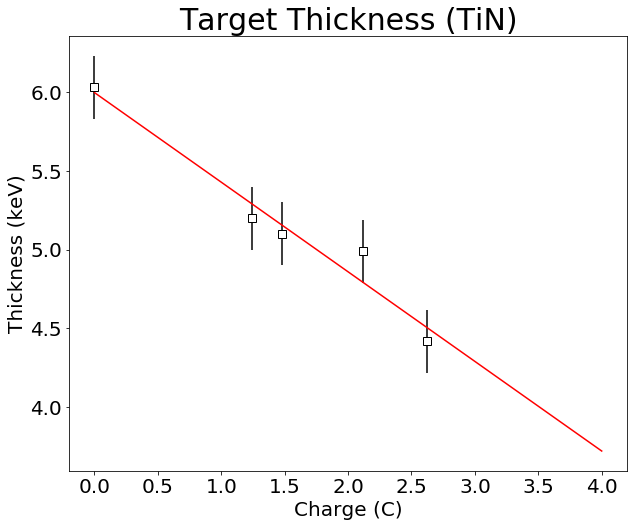
\includegraphics[width=\textwidth]{figures/targetThickness0.png}
            \caption[TiN sputtered target]%
            {{\small TiN sputtered target}}    
            \label{fig: target0}
        \end{subfigure}
        \hfill
        \begin{subfigure}[b]{0.475\textwidth}  
            \centering 
            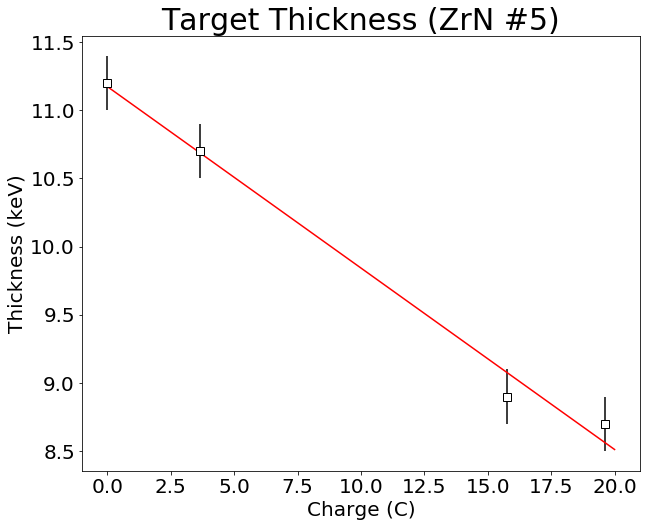
\includegraphics[width=\textwidth]{figures/targetThickness5.png}
            \caption[ZrN sputtered target 5]%
            {{\small ZrN sputtered target 5}}    
            \label{fig: target5}
        \end{subfigure}
        \vskip\baselineskip
        \begin{subfigure}[b]{0.475\textwidth}   
            \centering 
            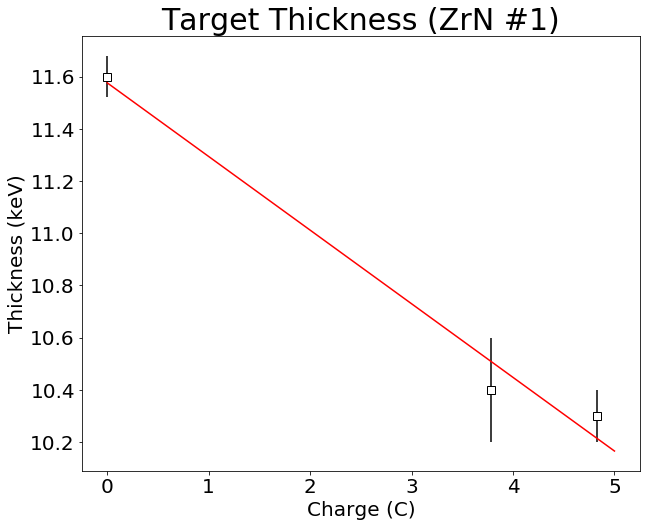
\includegraphics[width=\textwidth]{figures/targetThickness1.png}
            \caption[ZrN sputtered target 1]%
            {{\small ZrN sputtered target 1}}    
            \label{fig: target1}
        \end{subfigure}
        \quad
        \begin{subfigure}[b]{0.475\textwidth}   
            \centering 
            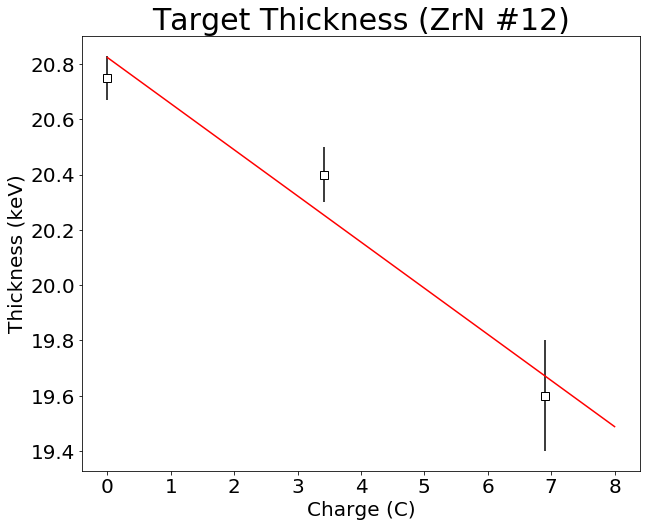
\includegraphics[width=\textwidth]{figures/targetThickness12.png}
            \caption[ZrN sputtered target 12]%
            {{\small ZrN sputtered target 12}}    
            \label{fig: target12}
        \end{subfigure}
        \caption[ The thicknesses of the various targets used in this experiment as a function of the charge delivered. This shows the deterioration of the targets through the course of the experiment where the thickness was monitored by scanning known resonances. ]
        {\small The thicknesses of the various targets used in this experiment as a function of the charge delivered. This shows the deterioration of the targets through the course of the experiment where the thickness was monitored by scanning known resonances. } 
        \label{fig: targetThicknesses}
\end{figure}




\section{Cross section determination}
\label{sec: cross-section}


In the following analysis, the differential cross section determination for each of the measured transitions follows the same procedure with the different individual correction factors for each of the transitions. Therefore, without loss of generality, they all occur according to the following procedure.

The yield of each transition, $Y_{i}$, is the number of reactions per incident projectile (protons, in this case). It was calculated by 

\begin{equation}
Y_{i} = \dfrac{N_{\gamma} C_{in}}{\eta N_{p} C_{out}},
\label{eqn: yieldCalc}
\end{equation}

\noindent where $N_{\gamma}$ is the measured number of $\gamma$-rays at the energy corresponding to the transition of interest, $C_{in}$ and $C_{out}$ are the summing in and out corrections, respectively, $N_{p}$ is the number of protons measured on target throughout the run, and $\eta$ is the detector efficiency at the measured $\gamma$ ray energy, $E_{\gamma}$. The uncertainty in this yield arises from the uncertainties in the counts of the $\gamma$-ray peak and the efficiency. In the case of the off-resonance region of the cross section, the uncertainty in the number of counts is the dominant term. These uncertainties are propagated through the yield calculation for each individual data point.

The experimental yield at a given incident proton energy, $Y(E_{p})$, corresponds to the differential cross section, $\dfrac{d \sigma}{d \Omega}$, integrated over the target thickness, $\Delta E$:

\begin{equation}
Y(E_{p}) = \int_{E_{p} - \Delta E}^{E_{p}} \dfrac{d \sigma(E)}{d \Omega} \dfrac{1}{\epsilon(E_{p})} dE,
\label{eqn: yieldCS}
\end{equation}

\noindent where, again, $\epsilon$ is the target's stopping power at the incident proton energy. 

For a thick target, the yield on top of a resonance can be written as

\begin{equation}
Y_{max}(\infty) = \dfrac{\lambda_{R}^{2}}{2} \dfrac{\omega \gamma}{\epsilon_{R}},
\end{equation}

\noindent where $\lambda_{R}$ is the de Broglie wavelength in the center-of-mass system and $\omega \gamma$ is the resonance strength. 



In determining the cross section for non-resonant regions, the thin target relation is useful because the cross section is approximately constant over the target thickness. The yield for such situation, then, becomes

\begin{equation}
Y_{NR}(E) = \dfrac{d \sigma}{d \Omega} \dfrac{\Delta(E_{p})}{\epsilon(E_{p})}
\end{equation}

\noindent where $\Delta(E_{p})$ is the target thickness in terms of energy for an incident beam of energy $E_{p}$ and NR denotes non-resonant. This can be rearranged in terms of the cross section

\begin{equation}
\dfrac{d \sigma}{d \Omega} = \dfrac{Y_{NR} \epsilon(E_{p})}{\Delta(E_{p})} = \dfrac{Y_{NR}}{N_{T}} = \dfrac{N_{\gamma}C_{in}} {\eta  N_{p} C_{out} N_{T}},
\label{eqn: thinTargetCS}
\end{equation}

\noindent where $N_{T}$ is the number of active target nuclei (in this case, nitrogen). In order to make calculations easier, this can be further reduced by factoring the infinitely-thick yield from resonance measurements by

\begin{eqnarray}
\dfrac{d \sigma}{d \Omega} &=& \dfrac{Y_{NR} \epsilon(E_{p})}{\Delta(E_{p})} \dfrac{Y_{max}(\infty)}{Y_{max}(\infty)} \\
   &=& \dfrac{\lambda_{R}^{2}}{2} \dfrac{\omega \gamma}{\epsilon_{R}} \dfrac{\epsilon(E_{p})}{\Delta(E_{p})} \dfrac{Y_{NR}}{Y_{max}(\infty)} \\
   &=& \dfrac{\lambda_{R}^{2}}{2} \dfrac{\omega \gamma}{\Delta(E_{p})} \dfrac{Y_{NR}}{Y_{max}(\infty)} 
\end{eqnarray}

\noindent This allows an experimental determination of the cross section by using only the de Broglie wavelength, which can be calculated from the experimental parameters, the resonance strength, which has been previously determined \cite{Imbriani2005, Daigle2016}, the target thickness, and the relative yields between non-resonant capture data with the yield on a known resonance (in this case, the $E_{p}$ = 278 keV resonance). 


This is the method by which the differential cross section of the $^{14}$N$\left( p,\gamma \right) ^{15}$O reaction was determined for the different transitions. The uncertainty on this differential cross section was calculated for each individual point by propagating the uncertainty in the number of nitrogen atoms with the uncertainty in the calculated yields. This also took into account the loss of nitrogen within the targets over the course of the experiment (see Sec.\ \ref{sec: targetCharacterization} for details). The resulting differential cross sections are shown in Figs.\ \ref{fig: cs679_targs} and \ref{fig: csGS_targs}. 



\begin{figure}
\thisfloatpagestyle{plain}
		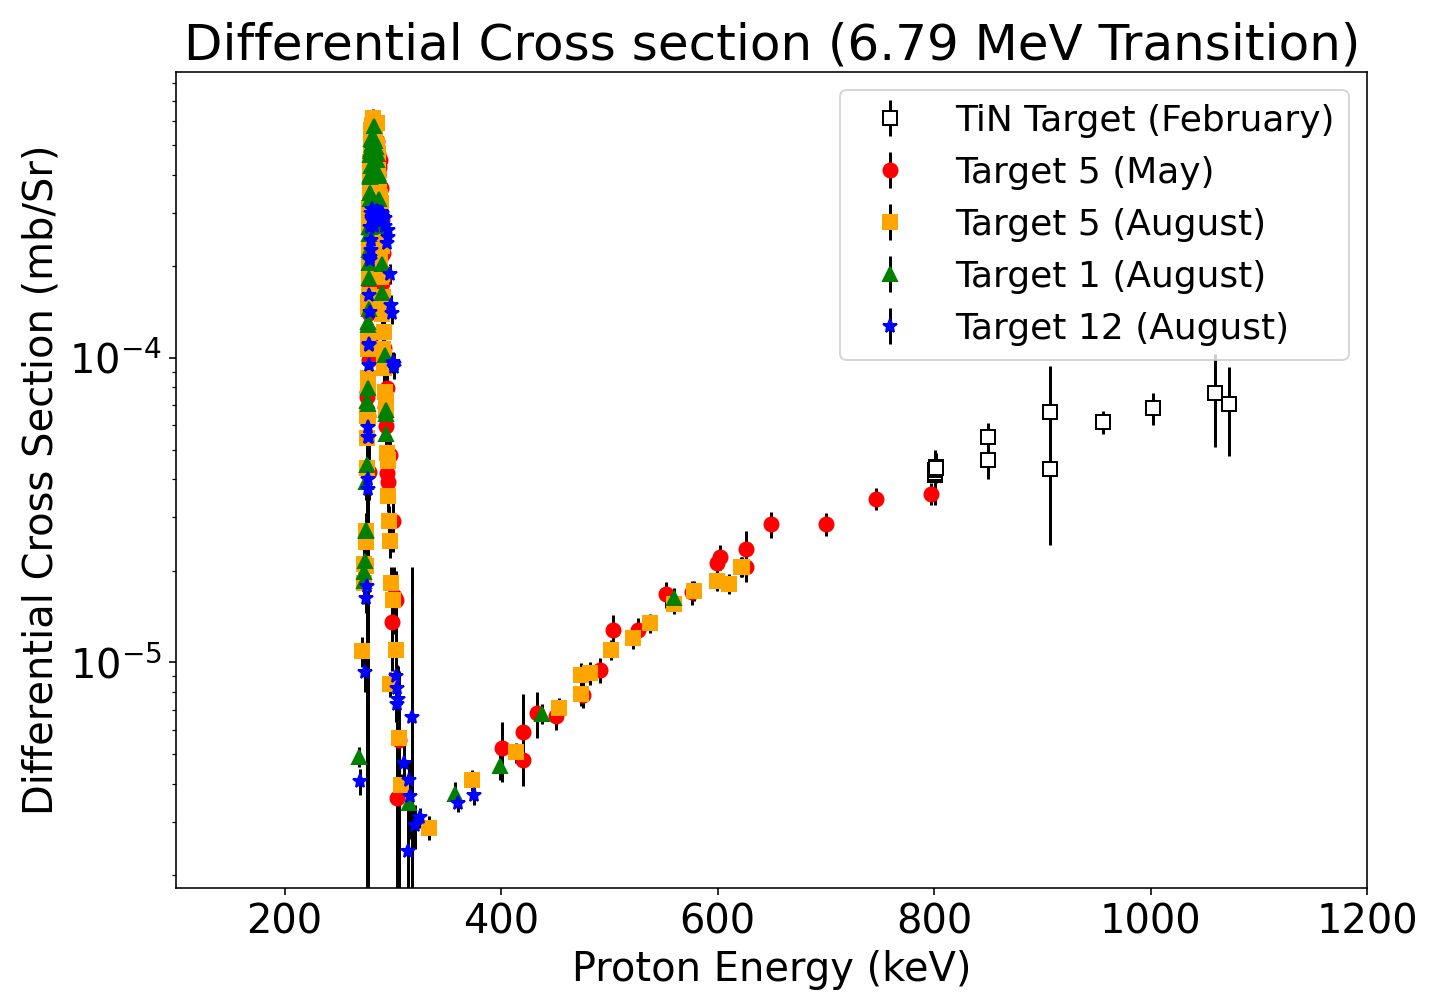
\includegraphics[width=1.0\linewidth]{figures/cs679_targs.png}
	\caption{Differential cross section for the 6.79 MeV transition in the $^{14}$N$\left( p,\gamma \right) ^{15}$O reaction, separated by the target used in measurements, showing the overlapping measurements and agreement between them. The target labels are nominal and do not represent the properties of the target, but targets 1 and 5 were the same thickness while target 12 was roughly double.}
	\label{fig: cs679_targs}
\end{figure}

\begin{figure}
\thisfloatpagestyle{plain}
		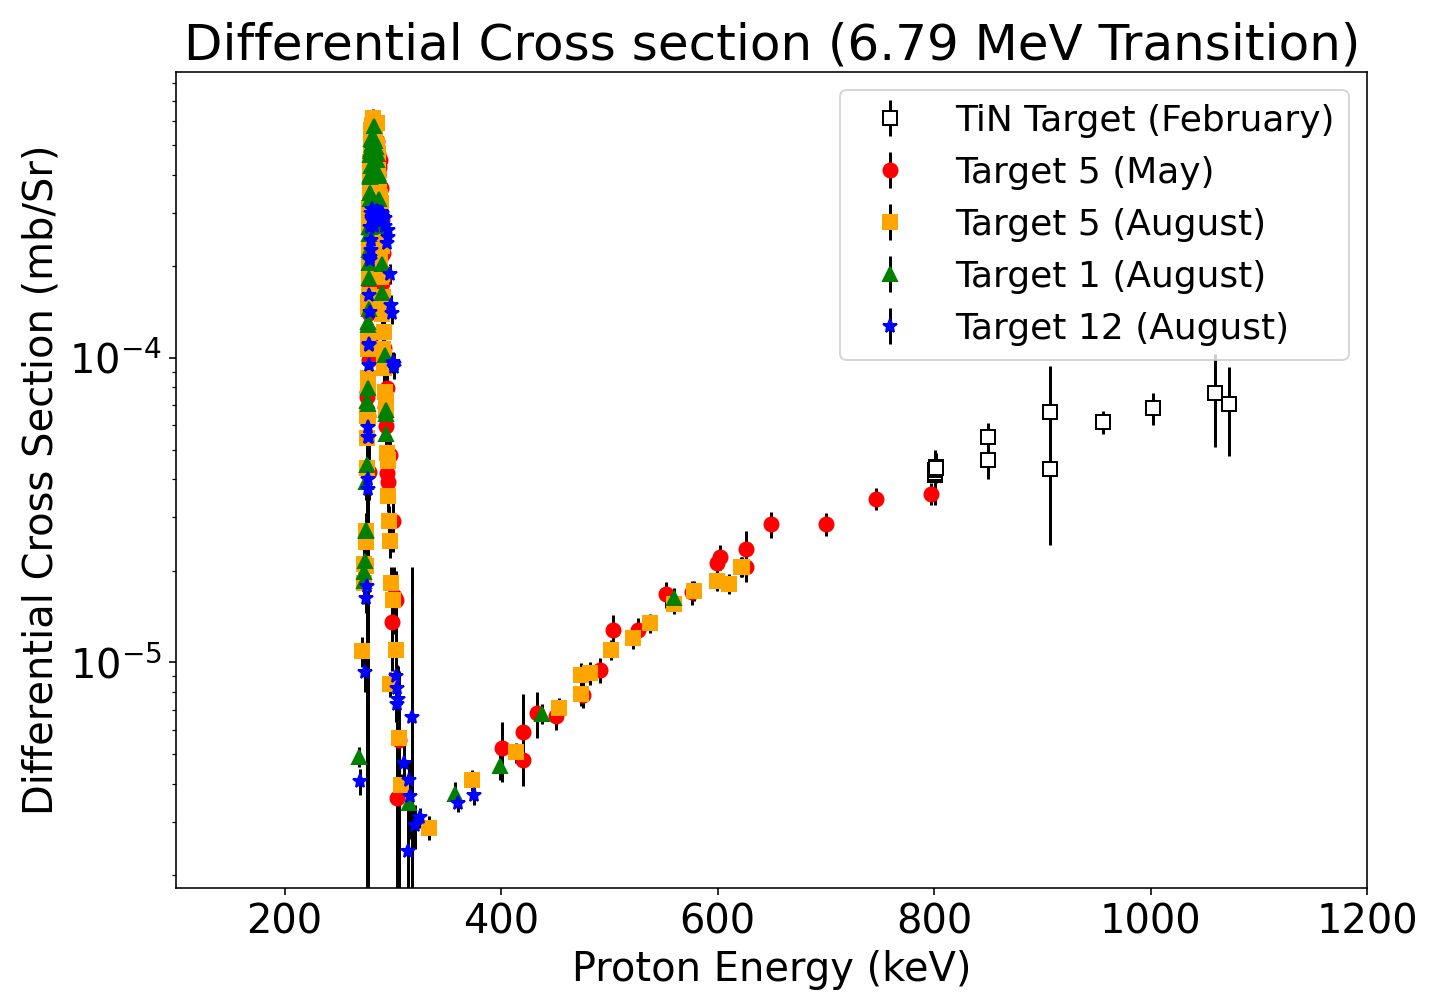
\includegraphics[width=1.0\linewidth]{figures/cs679_targs.png}
	\caption{Differential cross section for the ground state transition in the $^{14}$N$\left( p,\gamma \right) ^{15}$O reaction, separated by the target used in measurement, showing the overlapping measurements and agreement between them. The target labels are nominal and do not represent the properties of the target, but targets 1 and 5 were the same thickness while target 12 was roughly double. \textbf{BUT ACTUALLY GIVE THE FIGURE FOR THE GROUND STATE AND NOT THE 679 WHEN THE DATA HAVE BEEN SUMMING CORRECTED}.}
	\label{fig: csGS_targs}
\end{figure}




In order to move from differential measurements to a total cross section or total $S$-factor, as well as extrapolate to the Gamow window, an $R$-matrix calculations were performed with the \texttt{AZURE2} software \cite{Azuma2010}. A full description of this and incorporating the lifetime results into this analysis are presented later in Chapter \ref{chap: r-matrix}. Within the calculations, our data and the data from \citet{Li2016} are treated as differential. To compare our results alongside those from literature data \cite{Schroder1987, Imbriani2005, Runkle2005, Li2016, Wagner2018}, we scaled the resulting $S$-factors by $4\pi$ for plotting only.  These comparisons can be seen in the series of Figs.\ \ref{fig: full679} - \ref{fig: lowGS}. 


For the 6.79 MeV transition, the data are shown in Fig.~\ref{fig: full679} - \ref{fig: low679}. Our measurement agrees well with the data from \citet{Schroder1987} and \citet{Li2016} coming in from higher energies but is lower than the data from \citet{Wagner2018}. Our highest uncertainty data points overlap with the data from \citet{Wagner2018} but are otherwise discrepant. Our results agree well with the literature data in the lower-energy region where the results from LUNA \cite{Formicola2004, Imbriani2005, Marta2008, Marta2011} and LENA \cite{Runkle2005} made their measurements. Some of our data shows higher uncertainties at lower energies than other, measured data, but they agree well. Unlike the ground state data, the measurements for this transition stop at $\sim 1$ MeV. The runs at these energies were not done long enough to have appreciable statistics in the 6.79 peak. The resonance at this energy populates the ground state strongly and that was the focus of the measurement at those energies. This same lack of statistics is why the data points at 850 keV and 1000 keV also have comparatively larger uncertainties. These features can be seen highlighted in Fig.\ \ref{fig: highCompare679}, while the measured $S$-factor data for this transition in different energy regimes is plotted in Figs.\ \ref{fig: full679}, \ref{fig: highCompare679}, and \ref{fig: low679}.


\begin{figure}
\thisfloatpagestyle{plain}
		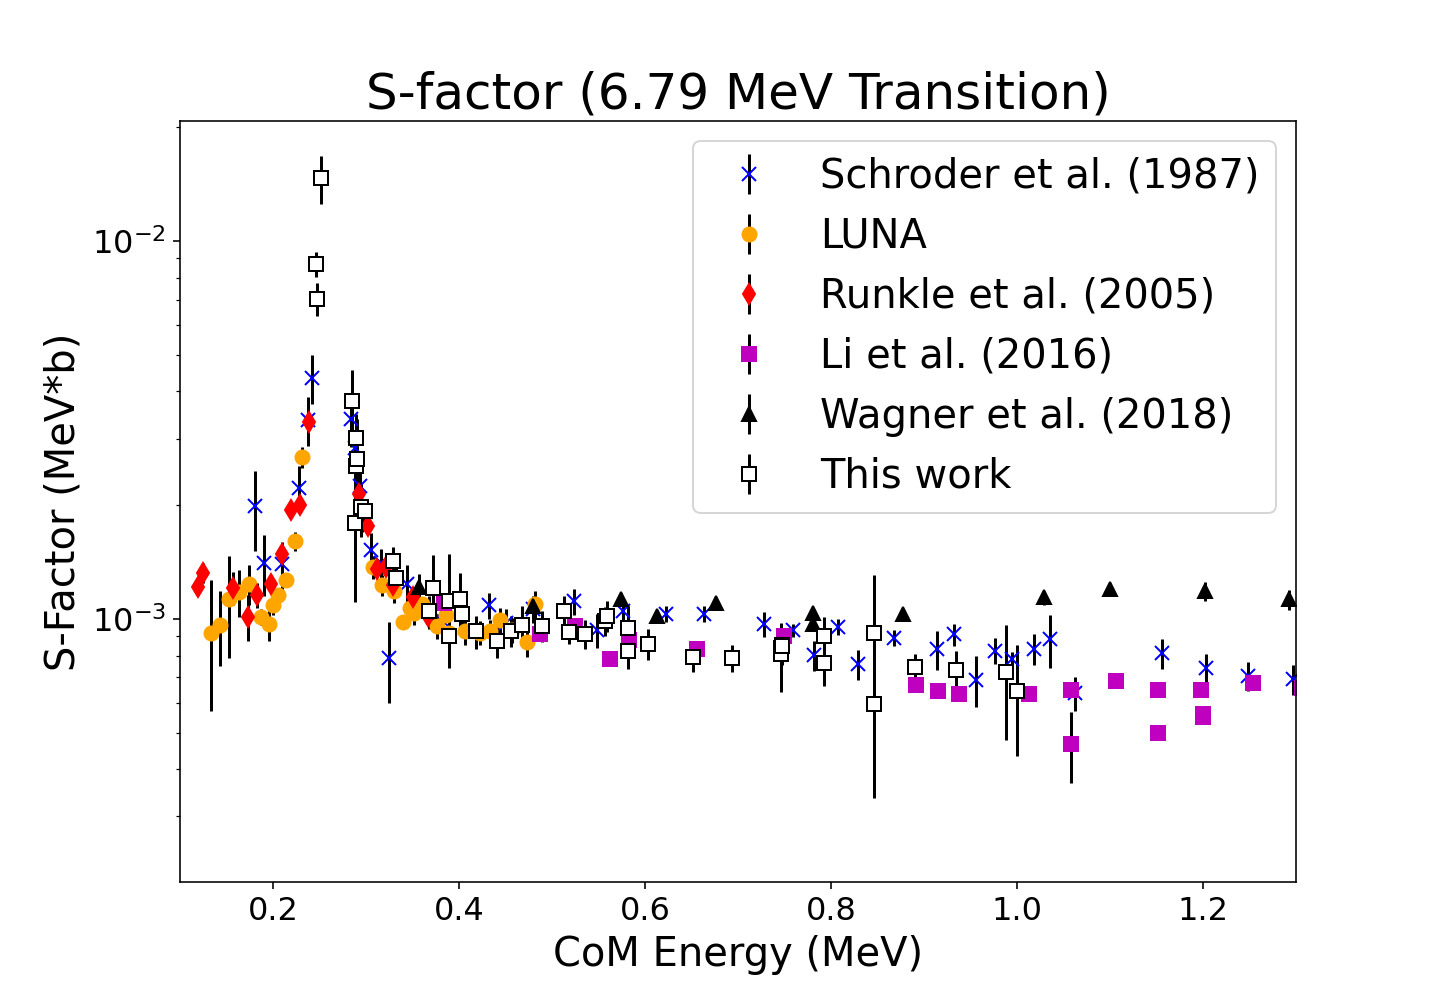
\includegraphics[width=1.0\linewidth]{figures/full679.png}
	\caption{$S$-factor for the 6.79 MeV transition in the $^{14}$N$\left( p,\gamma \right) ^{15}$O reaction for the entire energy range measured in this experiment. Also plotted are data from \cite{Schroder1987, Formicola2004, Imbriani2005, Runkle2005, Marta2008, Marta2011, Li2016, Wagner2018} for comparison. The LUNA data specifically represents the measurements \cite{Formicola2004, Imbriani2005, Marta2008, Marta2011}. Our data and that from \citet{Li2016} were both calculated as differential $S$-factors but scaled up by a factor of $4\pi$ for plotting purposes.  }
	\label{fig: full679}
\end{figure}

\begin{figure}
\thisfloatpagestyle{plain}
		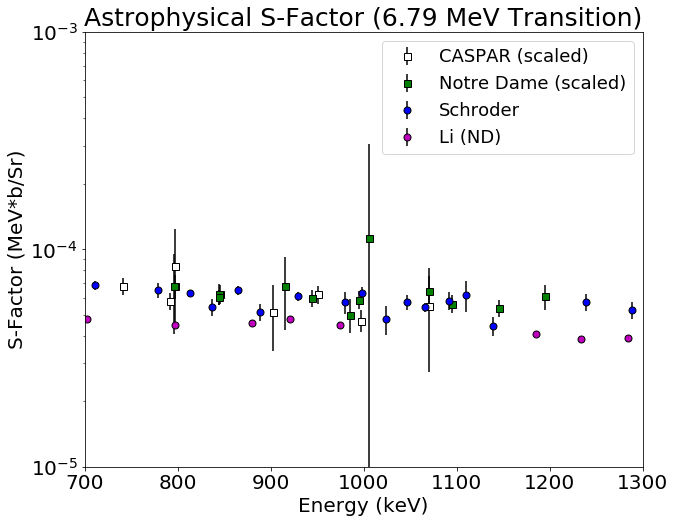
\includegraphics[width=1.0\linewidth]{figures/highCompare679.png}
	\caption{Differential cross section for the 6.79 MeV transition in the $^{14}$N$\left( p,\gamma \right) ^{15}$O reaction, highlighting the high energy region to compare the data taken at CASPAR to literature data in this region. The literature data plotted are taken from \cite{Schroder1987, Li2016, Wagner2018} for comparison. Our data and that from \citet{Li2016} were both calculated as differential $S$-factors but scaled up by a factor of $4\pi$ for plotting purposes.  }
	\label{fig: highCompare679}
\end{figure}

\begin{figure}
\thisfloatpagestyle{plain}
		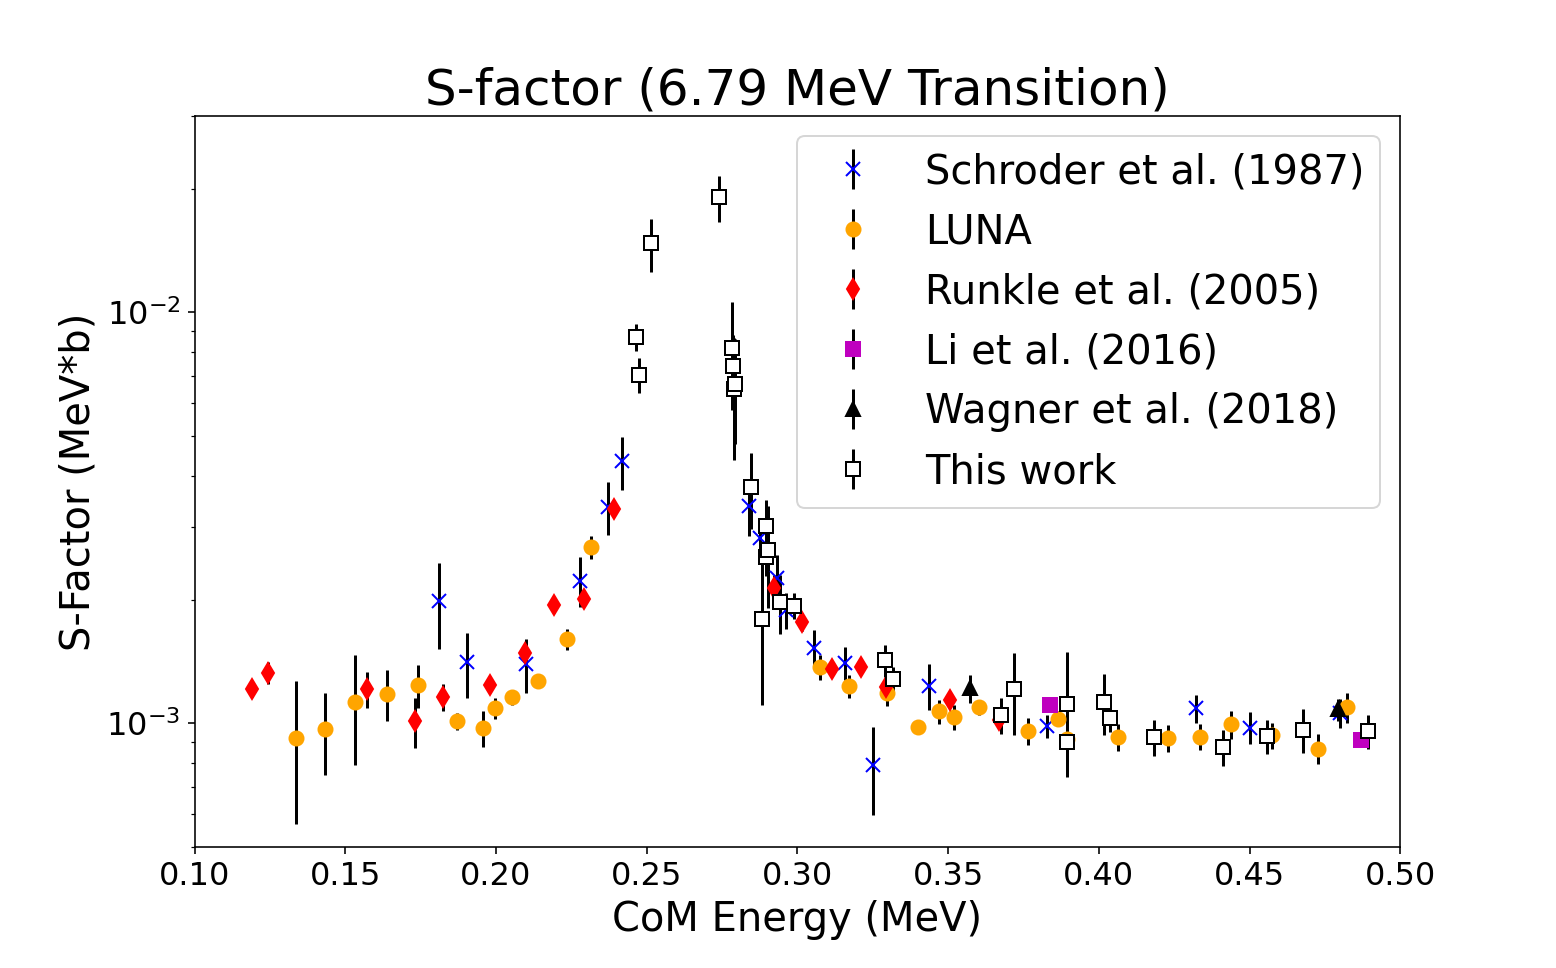
\includegraphics[width=1.0\linewidth]{figures/low679.png}
	\caption{Differential cross section for the 6.79 MeV transition in the $^{14}$N$\left( p,\gamma \right) ^{15}$O reaction, showing the behavior at low energy. Also plotted are data from \cite{Schroder1987, Formicola2004, Imbriani2005, Runkle2005, Marta2008, Marta2011, Li2016, Wagner2018} for comparison. The LUNA data specifically represents the measurements \cite{Formicola2004, Imbriani2005, Marta2008, Marta2011}. Our data and that from \citet{Li2016} were both calculated as differential $S$-factors but scaled up by a factor of $4\pi$ for plotting purposes. }
	\label{fig: low679}
\end{figure}

For the ground state transition, the data is shown in Figs.~\ref{fig: fullGS} - \ref{fig: lowGS}. \textbf{THE TREND IN THE DATA SHOWS THAT WE HAVE SOME RELATION TO PREVIOUS MEASUREMENTS. THERE IS SOME AGREEMENT MAYBE. I WILL GIVE MORE DISCUSSION TO THE GROUND STATE RESULTS HERE}. 

%Our measurement agrees well with the Schr{\"o}der data \cite{Schroder1987} and Li data \cite{Li2016} coming in from higher energies, with our measured $S$-factor dropping in the interference region between 300-400 keV to agree with the LUNA \cite{Imbriani2005} and LENA \cite{Runkle2005} data there. Our overall scale seems to be higher in the off resonance region, however, and only agrees with the highest energy data from the TUNL experiment \cite{Runkle2005}. Overall, this data shows significantly higher uncertainties at lower energies than the 6.79 MeV transition data. This is because this is a much more weakly populated transition and it was not feasible to run long enough to achieve appreciable statistics in the $\gamma$-ray data at these energies. Therefore, they have uncertainties dominated by the rate of measured $\gamma$'s in the experiment. The measured $S$-factor data for this transition is included in different energy regimes in Figs.\ \ref{fig: fullGS}, \ref{fig: highCompareGS}, \ref{fig: midGS}, and \ref{fig: lowGS}.

%Finally, with the 6.17 MeV transition, the data measured in this work show good agreement with other reported data. Unfortunately, at higher energies the data from our measurement have significantly larger uncertainties than the results reported by Ref.\ \cite{Schroder1987}. This is due primarily to two factors: this transition's peak appears on the shoulder of that of a background reaction in the spectrum, namely the $^{19}$F($p,\alpha \gamma$)$^{16}$O reaction, and it is by far the weakest transition measured, so it had the largest uncertainty in determining the peak area. The data from this transition is plotted in different energy regimes and included below as Figs.\ \ref{fig: full617}, \ref{fig: highCompare617}, and \ref{fig: low617}.





\begin{figure}
\thisfloatpagestyle{plain}
		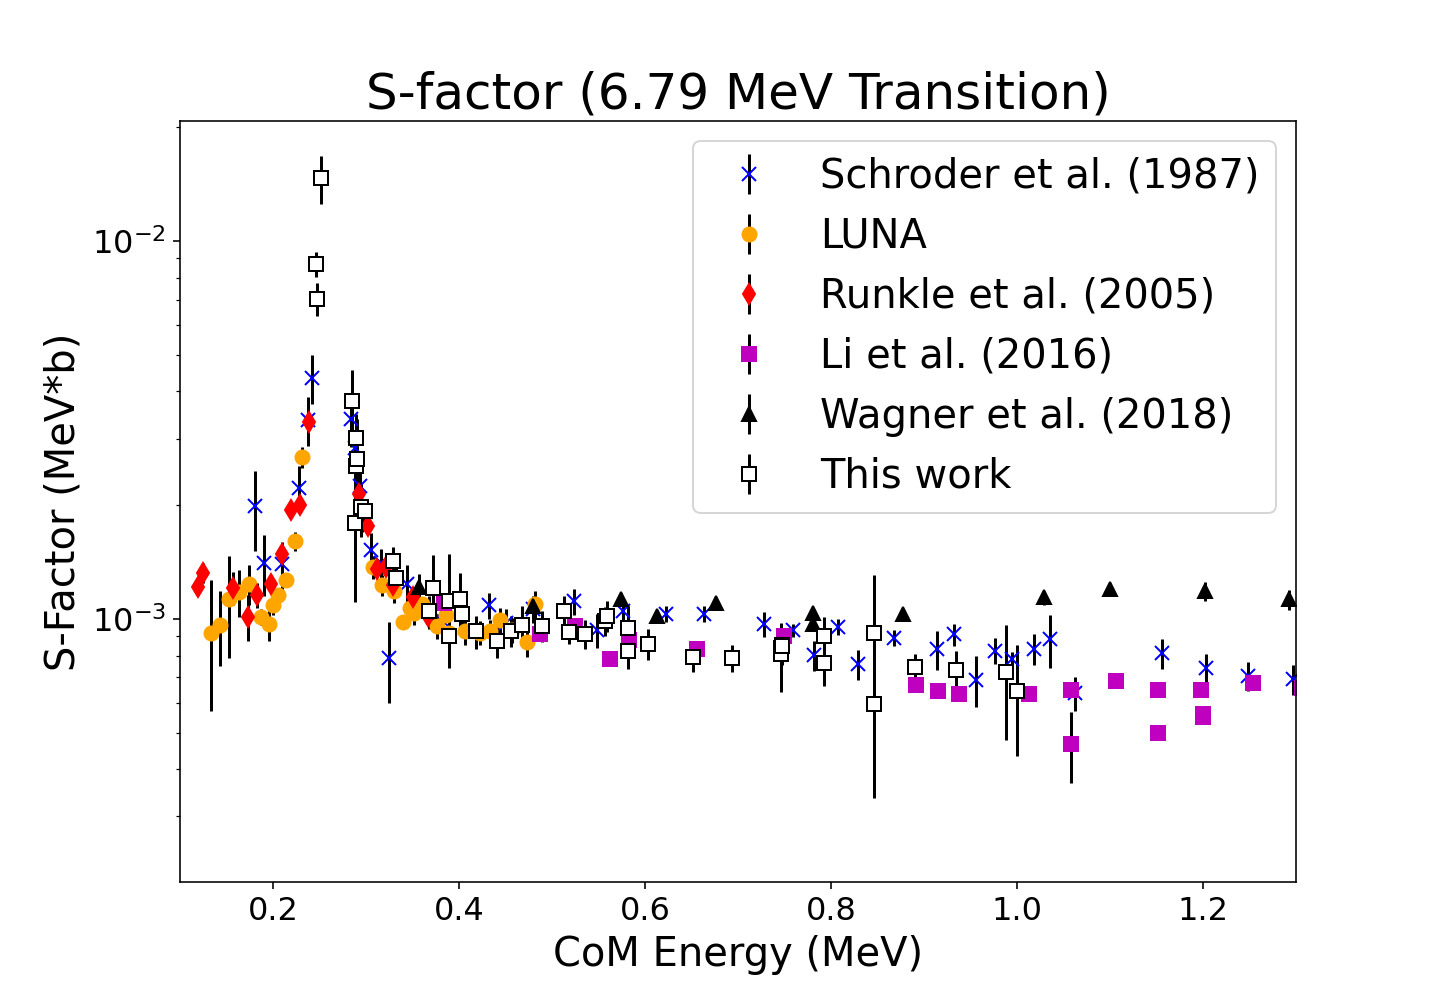
\includegraphics[width=1.0\linewidth]{figures/full679.png}
	\caption{Differential $S$-factor for the ground state transition in the $^{14}$N$\left( p,\gamma \right) ^{15}$O reaction for the entire energy range measured in this experiment. Also plotted are data from \cite{Schroder1987, Formicola2004, Imbriani2005, Runkle2005, Marta2008, Marta2011, Li2016, Wagner2018} for comparison. The LUNA data specifically represents the measurements \cite{Formicola2004, Imbriani2005, Marta2008, Marta2011}. Our data and that from \citet{Li2016} were both calculated as differential $S$-factors but scaled up by a factor of $4\pi$ for plotting purposes. \textbf{THIS FIGURE NEEDS TO BE UPDATED TO THE GROUND STATE WHEN THAT IS CALCULATED AFTER THE SUMMING CORRECTIONS.}}
	\label{fig: fullGS}
\end{figure}

%\begin{figure}
%\thisfloatpagestyle{plain}
%		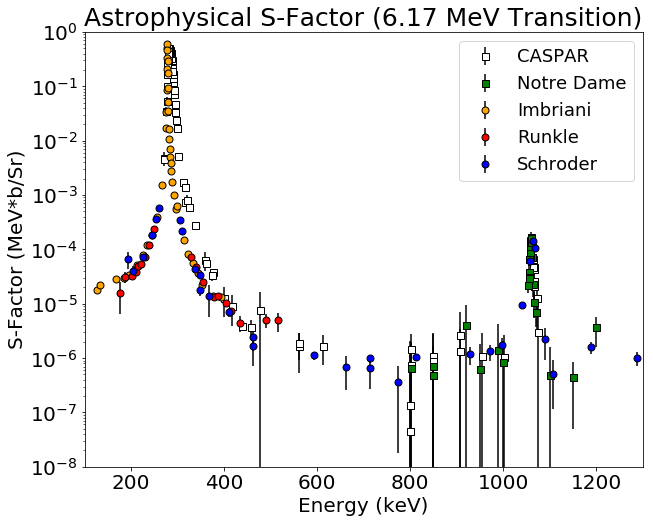
\includegraphics[width=1.0\linewidth]{figures/full617.png}
%	\caption{Differential $S$-factor for the 6.17 MeV transition in the $^{14}$N$\left( p,\gamma \right) ^{15}$O reaction for the entire energy range measured in this experiment. Also plotted are data from \cite{Schroder1987, Imbriani2005, Runkle2005, Li2016} for comparison.  }
%	\label{fig: full617}
%\end{figure}



\begin{figure}
\thisfloatpagestyle{plain}
		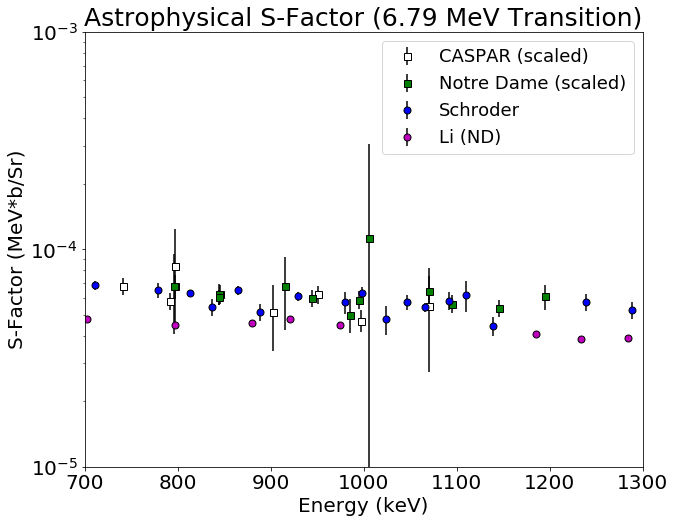
\includegraphics[width=1.0\linewidth]{figures/highCompare679.png}
	\caption{Differential cross section for the ground state transition in the $^{14}$N$\left( p,\gamma \right) ^{15}$O reaction highlighting the high energy region to compare the data taken at CASPAR to literature data in the same region. Also plotted are data from \cite{Schroder1987, Li2016, Wagner2018} for comparison. Our data and that from \citet{Li2016} were both calculated as differential $S$-factors but scaled up by a factor of $4\pi$ for plotting purposes.  \textbf{THIS FIGURE NEEDS TO BE UPDATED TO THE GROUND STATE WHEN THAT IS CALCULATED AFTER THE SUMMING CORRECTIONS.} }
	\label{fig: highCompareGS}
\end{figure}

%\begin{figure}
%\thisfloatpagestyle{plain}
%		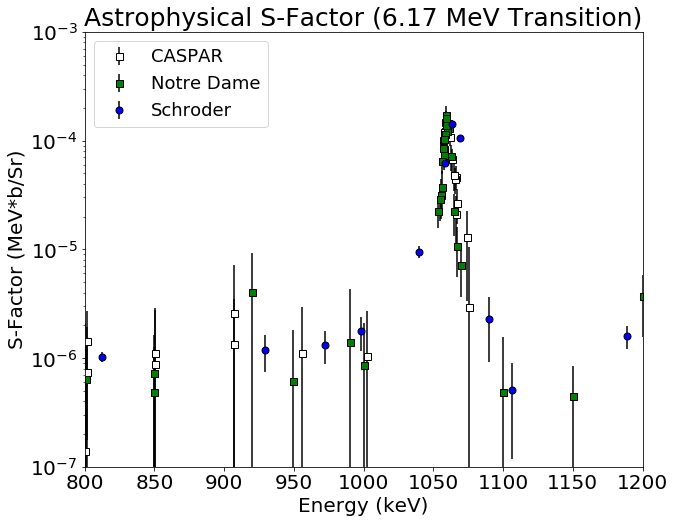
\includegraphics[width=1.0\linewidth]{figures/highCompare617.png}
%	\caption{Differential cross section for the 6.17 MeV transition in the $^{14}$N$\left( p,\gamma \right) ^{15}$O reaction highlighting the high energy region to compare the data taken at the NSL to CASPAR, showing the efficacy of the facility. Also plotted are data from \cite{Schroder1987, Li2016} for comparison.  }
%	\label{fig: highCompare617}
%\end{figure}


\begin{figure}
\thisfloatpagestyle{plain}
		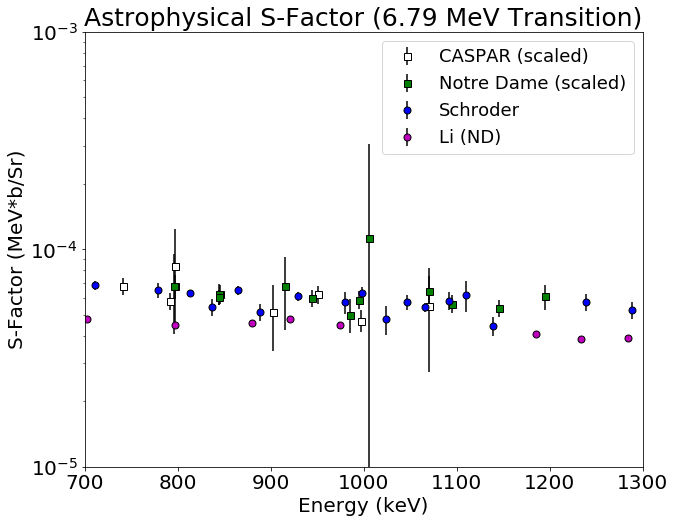
\includegraphics[width=1.0\linewidth]{figures/highCompare679.png}
	\caption{Differential cross section for the ground state transition in the $^{14}$N$\left( p,\gamma \right) ^{15}$O reaction, primarily detailing the off resonance region measured at CASPAR in this experiment. Also plotted are data from \cite{Schroder1987, Imbriani2005, Runkle2005, Li2016} for comparison. \textbf{THIS FIGURE NEEDS TO BE UPDATED TO THE GROUND STATE WHEN THAT IS CALCULATED AFTER THE SUMMING CORRECTIONS.}  }
	\label{fig: midGS}
\end{figure}



\begin{figure}
\thisfloatpagestyle{plain}
		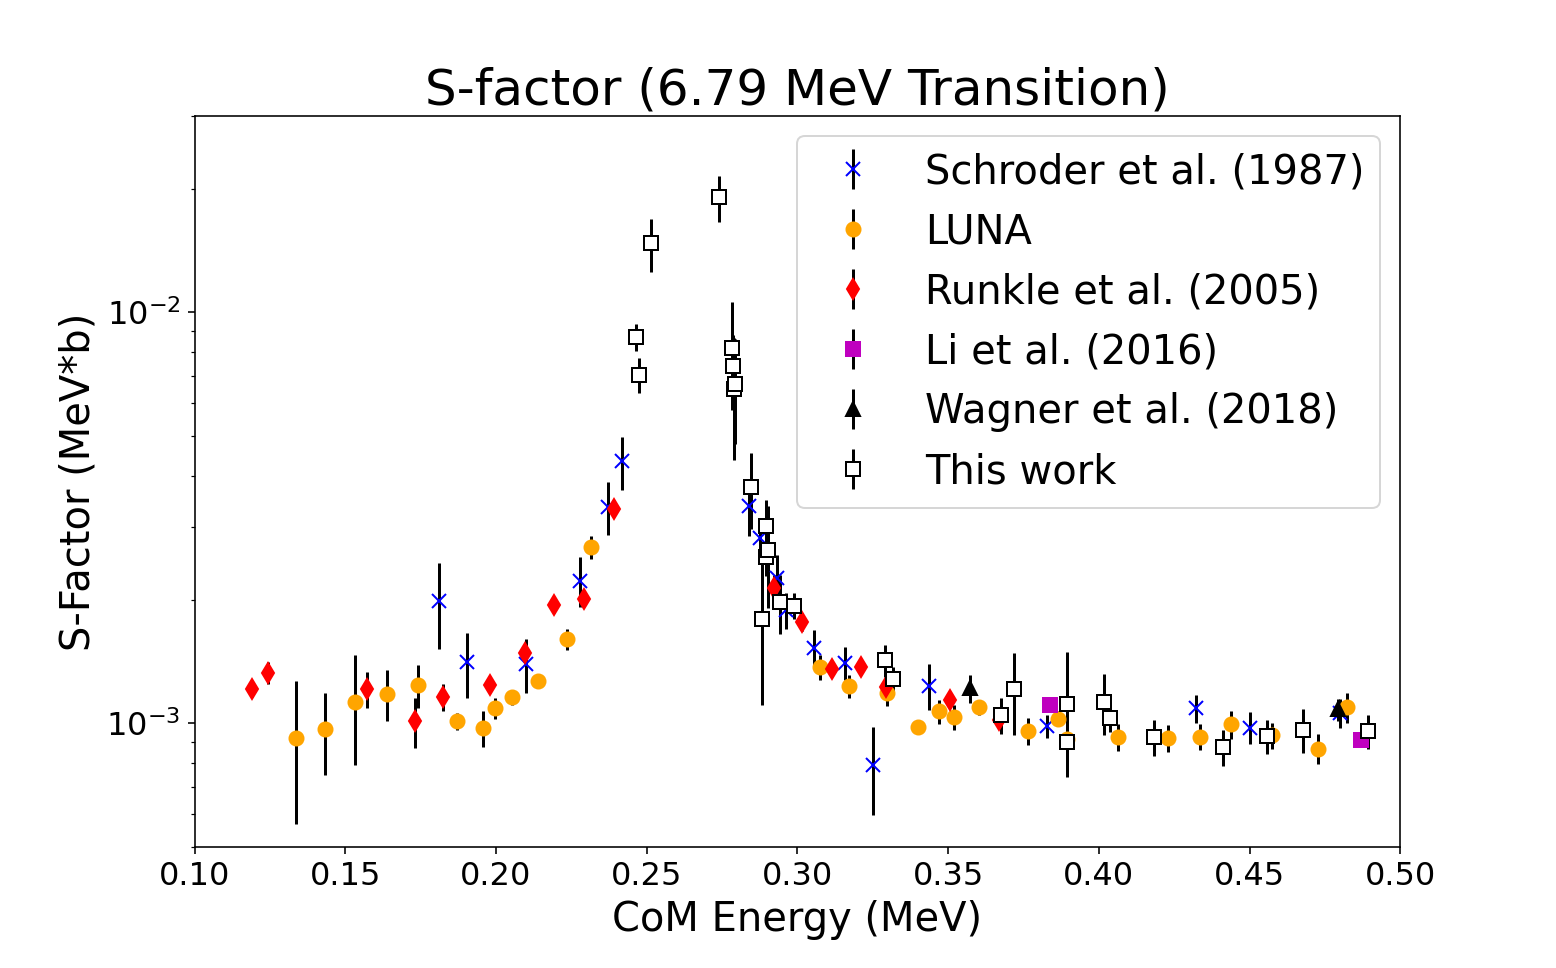
\includegraphics[width=1.0\linewidth]{figures/low679.png}
	\caption{Differential cross section for the ground state transition in the $^{14}$N$\left( p,\gamma \right) ^{15}$O reaction, showing the behavior of the $S$-factor at low energy. Also plotted are data from \cite{Schroder1987, Imbriani2005, Runkle2005, Li2016} for comparison. \textbf{THIS FIGURE NEEDS TO BE UPDATED TO THE GROUND STATE WHEN THAT IS CALCULATED AFTER THE SUMMING CORRECTIONS.} }
	\label{fig: lowGS}
\end{figure}

%\begin{figure}
%\thisfloatpagestyle{plain}
%		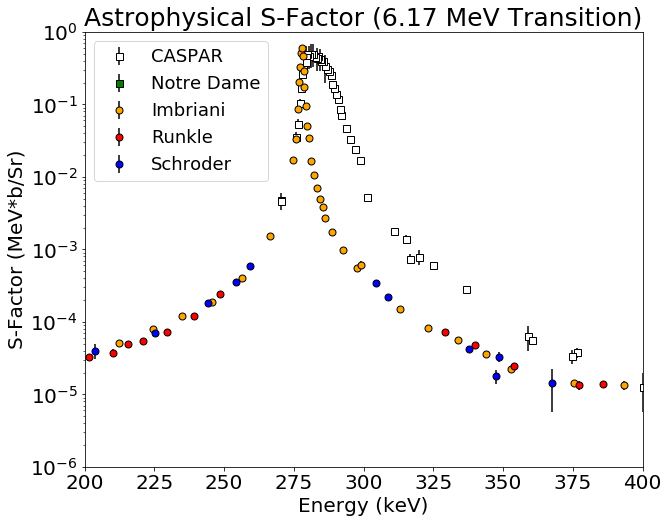
\includegraphics[width=1.0\linewidth]{figures/low617.png}
%	\caption{Differential cross section for the 6.17 MeV transition in the $^{14}$N$\left( p,\gamma \right) ^{15}$O reaction, showing the behavior of the $S$-factor at low energy. Also plotted are data from \cite{Schroder1987, Imbriani2005, Runkle2005, Li2016} for comparison. }
%	\label{fig: low617}
%\end{figure}

% % uncomment the following lines,
% if using chapter-wise bibliography
%
% \bibliographystyle{ndnatbib}
% \bibliography{example}
